\section{Structural Elements for MTConnectStreams}
\label{sec:Structural Elements for MTConnectStreams}
\lstset{numbers=left,xleftmargin=2em}

\glspl{structural element} are XML elements that form the logical structure for the \gls{mtconnectstreams} XML document.  These elements are used to organize the information and data that is reported by an \gls{agent} for a piece of equipment.  See \fig{streams-data-structure} for an overview of the \glspl{structural element} used in an \gls{mtconnectstreams} document.

The first, or highest level, \gls{structural element} in an \gls{mtconnectstreams} XML document is \gls{streams}. \gls{streams} is a container type XML element used to group the data reported from one or more pieces of equipment into a single XML document.  \gls{streams} \must always appear in the \gls{mtconnectstreams} document.

\gls{devicestream} is the next \gls{structural element} in the \gls{mtconnectstreams} document. \gls{devicestream} is also a XML container type element.   A separate \gls{devicestream} container is used to organize the information and data reported by each piece of equipment represented in the \gls{mtconnectstreams} document.  There \must be at least one \gls{devicestream} element in the \gls{streams} container.  

A \gls{devicestream} element provides the data reported by a piece of equipment.  Each \gls{devicestream} element \must contain the attributes \gls{name} and \gls{uuid} to correlate the \gls{devicestream} with a specific \gls{device} defined in the \gls{mtconnectdevices} document.  Once the \gls{devicestream} element is associated with a specific piece of equipment based on this identity, all data reported by that piece of equipment is directly associated with that unique identity and that association does not need to be repeated for every piece of data reported.  A client software application may then directly relate the information provided in the \gls{mtconnectdevices} document with the data provided in the \gls{mtconnectstreams} document based on this identity.

\gls{componentstream} is the next level XML element in the \gls{mtconnectstreams} document.  \gls{componentstream} is also a container type XML element.   There \must be a separate \gls{componentstream} XML element for each of the \glspl{structural element} (\gls{device} elements, \gls{top level} \gls{component} elements, or \gls{lower level} \gls{component} elements) defined for that piece of equipment in the associated \gls{mtconnectdevices} XML document.  A \gls{componentstream} representing a \gls{structural element} will only appear if there is data reported for that \gls{structural element}.  (Note:  See \citetitle{MTCPart2} of the MTConnect Standard for a description of the \glspl{structural element} for a piece of equipment).   

There are three (3) \glspl{structural element} – \gls{samples}, \gls{events}, and \gls{conditions} at the next level of the \gls{mtconnectstreams} document.  Each one of these \glspl{structural element} is a container type XML element.  These \glspl{structural element} group the data reported for each component of a piece of equipment according to the \gls{data entity} categories defined in \citetitle{MTCPart2}, Sections 7 and 8.  

\begin{itemize}

\item \gls{samples} contains \gls{sample category} category \glspl{data entity} defined in the \gls{mtconnectdevices} XML document (See \citetitle{MTCPart2}, Section 8.1)

\item \gls{events} contains \gls{event category} category \glspl{data entity} defined in the \gls{mtconnectdevices} XML document (See \citetitle{MTCPart2}, Section 8.2)

\item \gls{conditions} contains \gls{condition category} category \glspl{data entity} defined in the \gls{mtconnectdevices} XML document (See \citetitle{MTCPart2}, Section 8.3)
\end{itemize}

There \must be at least one of \gls{samples}, \gls{events}, or \gls{conditions} elements in each \gls{componentstream} container. 

\fig{streams-data-structure} XML tree structure illustrates the various \glspl{structural element} used to organize the data reported by a piece of equipment and the relationship between these elements. 

\begin{figure}[ht]
  \centering
  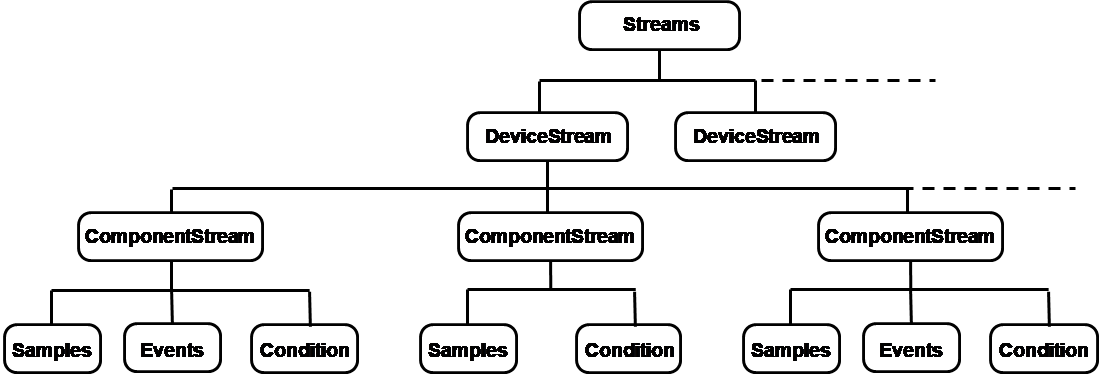
\includegraphics[width=1.0\textwidth]{figures/streams-data-structure.png}
  \caption{Streams Data Structure}
  \label{fig:streams-data-structure}
\end{figure}

\lst{example-of-devicestream} is a sample from an \gls{mtconnectstreams} XML document that contains the response from an \gls{agent} representing two pieces of equipment, \textit{mill-1} and \textit{mill-2}. The data from each piece of equipment is reported in a separate \gls{devicestream} container. 

\begin{lstlisting}[firstnumber=1,escapechar=|,%
    caption={Example of  DeviceStream},label={lst:example-of-devicestream}]
<MTConnectStreams ...>
  <Header ... />
  <Streams>
    <DeviceStream name="mill-1" uuid="1">
      <ComponentStream component="Device" name="mill-1"
          componentId="d1">
        <Events>
          <Availability dataItemId="avail1" name="avail"
              sequence="5"
              timestamp="2010-04-06T06:19:35.153141">
            AVAILABLE</Availability>
        </Events>
      </ComponentStream>
    </DeviceStream>
    <DeviceStream name="mill-2" uuid="2">
      <ComponentStream component="Device" name="mill-2"
          componentId="d2">
        <Events>
          <Availability dataItemId="avail2" name="avail" 
              sequence="15"
              timestamp="2010-04-06T06:19:35.153141">
            AVAILABLE</Availability>
        </Events>
      </ComponentStream>
    </DeviceStream>
  </Streams>
</MTConnectStreams>
\end{lstlisting}

In \lst{example-of-devicestream}, it should be noted that the \glspl{sequence number} are unique across the two pieces of equipment. Client software applications \MUSTNOT assume that the \gls{events} and \gls{samples} sequence numbers are strictly in sequence. All sequence numbers \MAYNOT be included. For instance, such a case would occur when HTTP filtering is applied to the request and the \gls{sample category}, \gls{event category}, and \gls{condition category} data types for other components are not returned. Another case would occur when an \gls{agent} is supporting more than one piece of equipment and data from only one piece of equipment is requested. Refer to MTConnect Standard \citetitle{MTCPart1}, \textit{Section 5} for more information on \glspl{sequence number}.


\subsection{Streams}

\gls{streams} is a container type XML element that \must contain only \gls{devicestream} elements.  \gls{streams} \may contain any number of \gls{devicestream} elements.  If there is no data to be reported for a request for data, an \gls{mtconnectstreams} document \must be returned with an empty \gls{streams} container.  \glspl{data entity} \maynot be directly associated with the \gls{streams} container.

The XML schema in \fig{streams-schema-diagram} represents the structure of the \gls{streams} XML element.   

\begin{figure}[ht]
  \centering
  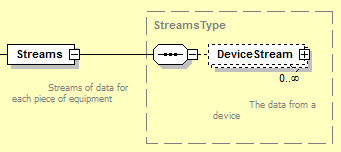
\includegraphics[width=0.75\textwidth]{figures/streams-schema-diagram.png}
  \caption{Streams Schema Diagram}
  \label{fig:streams-schema-diagram}
\end{figure}

\FloatBarrier

\tabulinesep = 5pt
\begin{longtabu} to \textwidth {
    |l|X[3l]|X[0.75l]|}
\caption{MTConnect Streams Element} \label{table:mtconnect-streams-element} \\

\hline
Element & Description & Occurrence \\
\hline
\endfirsthead

\hline
\multicolumn{3}{|c|}{Continuation of Table \ref{table:mtconnect-streams-element}}\\
\hline
Element & Description & Occurrence \\
\hline
\endhead

\gls{streams}
&
The first, or highest, level XML container element in an \gls{mtconnectstreams} \gls{response} Document provided by an \gls{agent} in response to a \gls{sample httprequest} or \gls{current httprequest} HTTP \gls{request}.
\newline There \MAY be only one \gls{streams} element in an \gls{mtconnectstreams}  \gls{response} Document for each piece of equipment represented in the document.
\newline An empty \gls{streams} container \MAY be provided to indicate that no data is available for the given \gls{request}.
\newline The \gls{streams} element \MAY contain any number of \gls{devicestream} elements, one for each piece of equipment represented in the \gls{mtconnectstreams} document.
&
1 \\ \hline

\end{longtabu}

\pagebreak

\subsection{DeviceStream}\label{sec:DeviceStream}

\gls{devicestream} is a XML container that organizes data reported from a single piece of equipment.  A \gls{devicestream} element \must be provided for each piece of equipment reporting data in an \gls{mtconnectstreams} document.

A \gls{devicestream} \may contain any number of \gls{componentstream} elements; limited to one for each component element represented in the \gls{mtconnectdevices} document.  If the response to the request for data from an \gls{agent} does not contain any data for a specific piece of equipment, an empty \gls{devicestream} element \may be created to indicate that the piece of equipment exists, but there was no data available.  In this case, there will be no \gls{componentstream} elements provided. 

\tabulinesep = 5pt
\begin{longtabu} to \textwidth {
    |l|X[3l]|X[0.75l]|}
\caption{MTConnect DeviceStream Element} \label{table:mtconnect-devicestream-element} \\

\hline
Element & Description & Occurrence \\
\hline
\endfirsthead

\hline
\multicolumn{3}{|c|}{Continuation of Table \ref{table:mtconnect-devicestream-element}}\\
\hline
Element & Description & Occurrence \\
\hline
\endhead

\gls{devicestream}
&
\glsentrydesc{devicestream}
\newline There \MAY be one or more \gls{devicestream} elements in a
\gls{streams} container; one for each piece of equipment represented in
the \gls{mtconnectstreams} document. 
&
0..* \\ \hline

\end{longtabu}

\subsubsection{XML Schema for DeviceStream}

The XML schema in \fig{devicestream-schema-diagram} represents the structure of the \gls{devicestream} XML element showing the attributes defined for \gls{devicestream} and the elements that \may be associated with \gls{devicestream}.

\begin{figure}[ht]
  \centering
  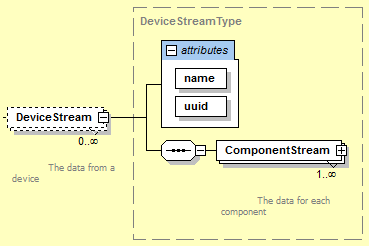
\includegraphics[width=0.7\textwidth]{figures/devicestream-schema-diagram.png}
  \caption{DeviceStream Schema Diagram}
  \label{fig:devicestream-schema-diagram}
\end{figure}
\FloatBarrier

\subsubsection{Attributes for DeviceStream}

\tbl{attributes-for-devicestream} defines the attributes that \must be provided to uniquely identify each specific piece of equipment associated with the information provided in each \gls{devicestream}.

\tabulinesep = 5pt
\begin{longtabu} to \textwidth {
    |l|X[3l]|X[0.75l]|}
\caption{Attributes for  DeviceStream} \label{table:attributes-for-devicestream} \\

\hline
Attribute & Description & Occurrence \\
\hline
\endfirsthead

\hline
\multicolumn{3}{|c|}{Continuation of Table \ref{table:attributes-for-devicestream}}\\
\hline
Attribute & Description & Occurrence \\
\hline
\endhead


\gls{name}
&
\glsentrydesc{name}
The \gls{name} associated with the piece of equipment reporting the data
contained in this \gls{devicestream} container.
\newline \gls{name} is a required attribute.
\newline The value reported for \gls{name} \MUST be the same as the value defined
for the \gls{name} attribute of the same piece of equipment in the
\gls{mtconnectdevices} document
\newline An \gls{nmtoken} XML type.
\newline \textbf{WARNING}: \gls{name} may become an optional attribute in future versions of the MTConnect Standard.
&
1 \\
\hline
 
\gls{uuid}
&
The \gls{uuid} associated with the piece of equipment reporting the data contained in this \gls{devicestream} container.
\newline \gls{uuid} is a required attribute. 
\newline The value reported for \gls{uuid} \MUST be the same as the value defined
for the \gls{uuid} attribute of the same piece of equipment in the
\gls{mtconnectdevices} document.
&
1 \\
\hline


\end{longtabu}

\subsubsection{Elements for DeviceStream}

\tbl{elements-for-devicestream} lists the XML element(s) that \may be provided in the \gls{devicestream} XML element.  

\tabulinesep = 5pt
\begin{longtabu} to \textwidth {
    |l|X[3l]|X[0.75l]|}
\caption{Elements for DeviceStream} \label{table:elements-for-devicestream} \\

\hline
Element & Description & Occurrence \\
\hline
\endfirsthead

\hline
\multicolumn{3}{|c|}{Continuation of Table \ref{table:elements-for-devicestream}}\\
\hline
Element & Description & Occurrence \\
\hline
\endhead
 
\gls{componentstream}
&
\glsentrydesc{componentstream}
\newline Any number of \gls{componentstream} elements \MAY be provided
in a \gls{devicestream} container.
\newline There \MUST be a separate \gls{componentstream} XML element
for each of the \glspl{structural element} (\gls{device} elements, \gls{top level}
\gls{component} elements, or \gls{lower level} \gls{component} elements)
defined for that piece of equipment in the associated \gls{mtconnectdevices} XML document. A \gls{componentstream}
representing a \gls{structural element} will only appear if there is data reported for that \gls{structural element}. 
&
0..* \\
\hline

\end{longtabu}

\subsection{ComponentStream}\label{sec:ComponentStream}

\gls{componentstream} is a XML container that organizes the data associated with each \gls{structural element} (\gls{device} element, \gls{top level} \gls{component}, or \gls{lower level} \gls{component} element) defined for that piece of equipment in the associated \gls{mtconnectdevices} XML document.  The data reported in each \gls{componentstream} element \must be grouped into individual XML containers based on the value of the \gls{category} attribute (\gls{sample category}, \gls{event category}, or \gls{condition category}) defined for each \gls{data entity} in the \gls{mtconnectdevices} XML document.  These containers are \gls{samples}, \gls{events}, and \gls{conditions}.   

\subsubsection{XML Schema for ComponentStream}

The XML schema in \fig{componentstream-schema-diagram} represents the structure of a \gls{componentstream} XML element showing the attributes defined for \gls{componentstream} and the elements that \may be associated with \gls{componentstream}.

\begin{figure}[ht]
  \centering
  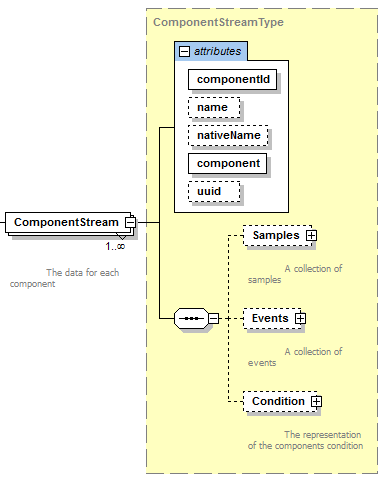
\includegraphics[width=0.7\textwidth]{figures/componentstream-schema-diagram.png}
  \caption{ComponentStream Schema Diagram}
  \label{fig:componentstream-schema-diagram}
\end{figure}

\FloatBarrier

\gls{componentstream} is similar to \gls{devicestream} in that the attributes uniquely identify the \gls{structural element} with which the data reported is directly associated.  This information does not have to be repeated for each \gls{data entity}.   In the case of the \gls{devicestream}, the attributes uniquely identify the piece of equipment associated with the data.   In the case of the \gls{componentstream}, the attributes identify the specific \gls{structural element} within a piece of equipment associated with each \gls{data entity}.  

\subsubsection{Attributes for ComponentStream}

The \tbl{attributes-for-componentstream} defines the attributes used to uniquely identify the specific \gls{structural element}(s) of a piece of equipment associated with the data reported in the \gls{mtconnectstreams} document.  


\tabulinesep = 5pt
\begin{longtabu} to \textwidth {
    |l|X[3l]|X[0.75l]|}
\caption{Attributes for ComponentStream} \label{table:attributes-for-componentstream} \\

\hline
Attribute & Description & Occurrence \\
\hline
\endfirsthead

\hline
\multicolumn{3}{|c|}{Continuation of Table \ref{table:attributes-for-componentstream}}\\
\hline
Attribute & Description & Occurrence \\
\hline
\endhead
 
\gls{componentid} 
&
The identifier of the \gls{structural element} (\gls{device} element, \gls{top level} \gls{component} element, or \gls{lower level} \gls{component} element) as defined by the \gls{id} attribute of the corresponding \gls{structural element} in the \gls{mtconnectdevices} XML document.
\newline \gls{componentid} is a required attribute.
\newline The identifier \MUST be the same as that defined in the \gls{mtconnectdevices} document to associate the data reported in the \gls{componentstream} container with the \gls{structural element} identified
in the \gls{mtconnectdevices} document.
&
1 \\
\hline


\gls{name}
&
The name of the \gls{componentstream} element.
\newline \gls{name} is an optional attribute.
\newline If \gls{name} is not defined for a specific \gls{structural element} in the
\gls{mtconnectdevices} document, it \MUSTNOT be provided for the corresponding \gls{componentstream} element in the \gls{mtconnectstreams} document.
\newline If \gls{name} is defined for a specific \gls{structural element} in the \gls{mtconnectdevices} document, it \MAY be provided for the corresponding \gls{componentstream} element in the \gls{mtconnectstreams} document.
\newline If provided, the value reported for name \MUST be the same as the
value defined for the name attribute of the corresponding \gls{structural element} (\gls{device} element, \gls{top level} \gls{component} element, or \gls{lower level} \gls{component} element) defined in the \gls{mtconnectdevices} XML document.
\newline An \gls{nmtoken} XML type.
&
0..1 \\
\hline

\gls{nativename}
&
\gls{nativename} identifies the common name normally associated with
the \gls{componentstream} element.
\newline \gls{nativename} is an optional attribute.
\newline If \gls{nativename} is not defined for a specific \gls{structural element} in the \gls{mtconnectdevices} document, it \MUSTNOT be provided for the
corresponding \gls{componentstream} element in the
\gls{mtconnectstreams} document.
\newline If \gls{nativename} is defined for a specific \gls{structural element} in the
\gls{mtconnectdevices} document, it \MAY be provided for the
corresponding \gls{componentstream} element in the
\gls{mtconnectstreams} document.
\newline If provided, the value reported for \gls{nativename} \MUST be the same as the value defined for the \gls{nativename} attribute of the corresponding
\gls{structural element} (\gls{device} element, \gls{top level} \gls{component} element,
or \gls{lower level} \gls{component} element) defined in the
\gls{mtconnectdevices} XML document.
&
0..1 \\
\hline

\gls{component componentstream}
&
\gls{component componentstream} identifies the \gls{structural element} (\gls{device}, \gls{top level} \gls{component}, or \gls{lower level} \gls{component}) associated with the
\gls{componentstream} element.
\newline \gls{component componentstream} is a required attribute.
\newline The value reported for component \MUST be the same as the value
defined for the Element Name of the XML container representing the
corresponding \gls{structural element} (\gls{device} element, \gls{top level}
\gls{component} element, or \gls{lower level} \gls{component} element) defined in
the \gls{mtconnectdevices} XML document.
\newline Examples of \gls{component} are \gls{device}, \gls{axes}, \gls{controller},
\gls{linear}, \gls{electric} and \gls{loader}.
&
1 \\
\hline

\gls{uuid}
&
\gls{uuid} of the \gls{componentstream} element.
\newline \gls{uuid} is an optional attribute.
\newline If \gls{uuid} is not defined for a specific \gls{structural element} in the
\gls{mtconnectdevices} document, it \MUSTNOT be provided for the
corresponding \gls{componentstream} element in the
\gls{mtconnectstreams} document.
\newline If \gls{uuid} is defined for a specific \gls{structural element} in the
\gls{mtconnectdevices} document, it \MAY be provided for the
corresponding \gls{componentstream} element in the
\gls{mtconnectstreams} document, but it is not required.
\newline If provided, the value reported for \gls{uuid} \MUST be the same as the
value defined for the \gls{uuid} attribute of the corresponding \gls{structural element} (\gls{device} element, \gls{top level} \gls{component} element, or \gls{lower level} \gls{component} element) defined in the \gls{mtconnectdevices}
XML document.
&
0..1 \\
\hline


\end{longtabu}

\subsubsection{Elements for ComponentStream}

In the \gls{componentstream} container, an \gls{agent} \must organize the data reported in each \gls{componentstream} into individual \gls{samples}, \gls{events}, or \gls{conditions} XML containers based on the value of the \gls{category} attribute (i.e., \gls{sample category}, \gls{event category}, or \gls{condition category}) defined for each \gls{data entity} defined in the \gls{mtconnectdevices} XML document.

Each \gls{componentstream} element \must include at least one \gls{events}, \gls{samples}, or \gls{conditions} XML container element.   \glspl{data entity} returned in each of the \gls{componentstream} container elements are defined in the \tbl{elements-for-componentstream}. 

\tabulinesep = 5pt
\begin{longtabu} to \textwidth {
    |l|X[3l]|X[0.75l]|}
\caption{Elements for ComponentStream} \label{table:elements-for-componentstream} \\

\hline
Element & Description & Occurrence \\
\hline
\endfirsthead

\hline
\multicolumn{3}{|c|}{Continuation of Table \ref{table:elements-for-componentstream}}\\
\hline
Element & Description & Occurrence \\
\hline
\endhead

\gls{samples}
&
An XML container type element.
\newline \gls{samples} organizes the \gls{sample category} type \glspl{data entity} defined in the \gls{mtconnectdevices} document that are reported in each
\gls{componentstream} XML element.
&
0..1 \notesign \\
\hline

\gls{events}
&
An XML container type element.
\newline \gls{events} organizes the \gls{event category} type \glspl{data entity} defined in the \gls{mtconnectdevices} document that are reported in each
\gls{componentstream} XML element.
&
0..1 \notesign \\
\hline

\gls{conditions}
&
An XML container type element.
\newline \gls{conditions} organizes the \gls{condition category} type \glspl{data entity} defined in the \gls{mtconnectdevices} document that are reported in each
\gls{componentstream} XML element.
&
0..1 \notesign \\
\hline

\end{longtabu}

\begin{note}
Note: \notesign The \gls{componentstream} element \must contain at least one of these element types.

\end{note}

\section{Data Entities}\label{sec:Data Entities}

When a piece of equipment reports values associated with \gls{dataitem} elements defined in the \gls{mtconnectdevices} document, that information is organized as \glspl{data entity} in the \gls{mtconnectstreams} document.   These \glspl{data entity} are organized in containers within each \gls{componentstream} element based on the \gls{category} attribute defined for the corresponding \gls{dataitem} in the \gls{mtconnectdevices} document:

\tab \gls{dataitem} elements defined with a \gls{category} attribute of \gls{sample category} in the \gls{mtconnectdevices} document are mapped to the \gls{samples} XML container in the associated \gls{componentstream} element.

\tab \gls{dataitem} elements defined with a \gls{category} attribute of \gls{event category} in the \gls{mtconnectdevices} document are mapped to the \gls{events} XML container in the associated \gls{componentstream} element.

\tab \gls{dataitem} elements defined with a \gls{category} attribute of \gls{condition category} in the \gls{mtconnectdevices} document are mapped to the \gls{conditions} XML container in the associated \gls{componentstream} element.

The XML tree in \fig{componentstream-xml-tree-diagram} demonstrates how \glspl{data entity} are organized in these containers.  

\begin{figure}[ht]
  \centering
  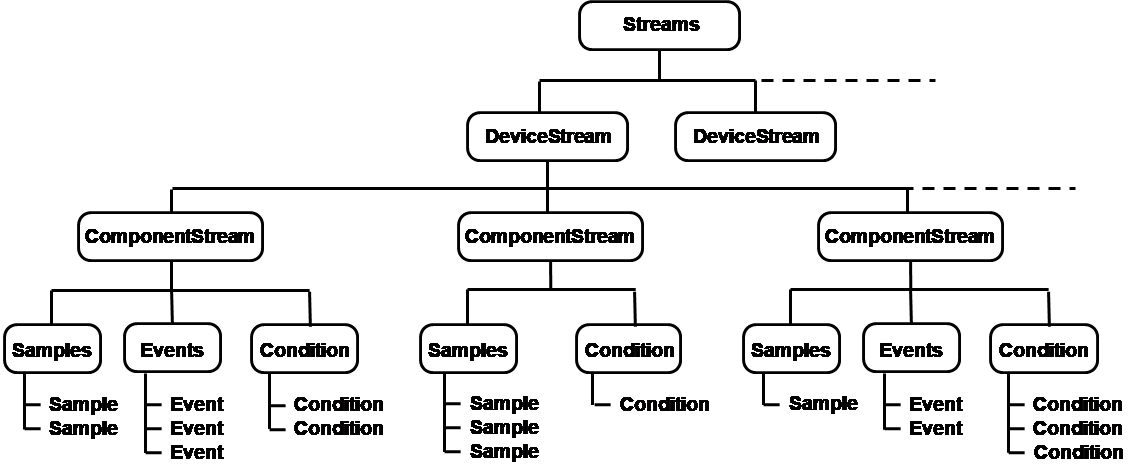
\includegraphics[width=1.0\textwidth]{figures/componentstream-xml-tree-diagram.png}
  \caption{ComponentStream XML Tree Diagram}
  \label{fig:componentstream-xml-tree-diagram}
\end{figure}
\FloatBarrier

\lst{example-of-mtconnectstreams} is an illustration of the structure of an XML document demonstrating how \glspl{data entity} are reported in a \gls{mtconnectstreams} document:

\newpage

\begin{lstlisting}[firstnumber=1,escapechar=|,%
    caption={Example of  MTConnectStreams},label={lst:example-of-mtconnectstreams}]
<MTConnectStreams>
  <Header/>
  <Streams>
    <DeviceStream>
      <ComponentStream>
        <Samples>
          <Sample/>
          <Sample/>
        </Samples>
        <Events>
          <Event/>
          <Event/>
        </Events>
        <Condition>
          <Condition/>
          <Condition/>
        </Condition>
      </ComponentStream>
      <ComponentStream>
        <Samples>
          <Sample/>
          <Sample/>
        </Samples>
        <Events>
          <Event/>
          <Event/>
        </Events>
        <Condition>
          <Condition/>
          <Condition/>
        </Condition>
      </ComponentStream>
    </DeviceStream>
  </Streams>
</MTConnectStreams>
\end{lstlisting}

\begin{note}
Note: There are no specific requirements defining the sequence in which the \gls{componentstream} XML elements are organized in the \gls{mtconnectstreams} document.  They \may be organized in any sequence based on the implementation of an \gls{agent}.  The sequence in which the \gls{componentstream} XML elements appear does not impact the ability for a client software application to interpret the information that it receives in the document.

\end{note}

When an \gls{agent} responds to a  \gls{current httprequest} HTTP request, the information returned in the \gls{mtconnectstreams} document \must include the most current value for every \gls{data entity} defined in the \gls{mtconnectdevices} document subject to any filtering included within the request.

When an \gls{agent} responds to a \gls{sample httprequest} HTTP request, the information returned in the \gls{mtconnectstreams} document \must include the occurrences for each \gls{data entity} that are available to an \gls{agent} subject to filtering and the count parameter included within the request (see \citetitle{MTCPart1} for a full definition of the protocol). 

\subsection{Element Names for Data Entities}

In the \gls{mtconnectdevices} document, \glspl{data entity} are grouped as \gls{dataitem} XML elements within each \gls{device}, \gls{top level} \gls{component}, and \gls{lower level} \gls{component} \gls{structural element}.  The \glspl{data entity} reported in the \gls{mtconnectstreams} document associated with each of these \glspl{structural element} are represented with an \gls{element name} based on the \gls{category} and \gls{type} defined for each of the \gls{dataitem} elements in the \gls{mtconnectdevices} document.

\subsubsection{Element Names when MTConnectDevices category is SAMPLE or EVENT}

The \glspl{data entity} reported in the \gls{mtconnectstreams} document associated with each \gls{dataitem} element defined in the \gls{mtconnectdevices} document with a \gls{category} attribute of \gls{sample category} or \gls{event category} \must be identified in the \gls{mtconnectstreams} document with an \gls{element name} derived from the \gls{type} attribute defined for that \gls{dataitem} element in the \gls{mtconnectdevices} document.

\lst{example-of-dataitem-in-mtconnectdevices} describes the most common method used to derive the \gls{element name} for a \gls{data entity} reported in the \gls{mtconnectstreams} document from the information describing that \gls{dataitem} element in the \gls{mtconnectdevices} document:

\ulheading{DataItem Represented in the MTConnectDevices Document}

\begin{lstlisting}[firstnumber=1,escapechar=|,%
    caption={DataItem Represented in MTConnectDevices Document},label={lst:example-of-dataitem-in-mtconnectdevices}]
<DataItem type="AXIS_FEEDRATE" id="xf" name="Xfrt"
    category="SAMPLE" units="MILLIMETER/SECOND"
    nativeUnits="MILLIMETER/SECOND/>
\end{lstlisting}

\begin{itemize}
\item \gls{dataitem}:  The XML \gls{element name} for this \gls{data entity}.  

\begin{note}
Note:  \gls{element name} must not be confused with the name attribute for the data item element.

\end{note}

\item \gls{type}, \gls{category}, \gls{units}, and \gls{nativeunits}:  Attributes that provide additional information regarding each data item in the \gls{mtconnectdevices} document.  
\end{itemize}

\ulheading{Response Format reported in the MTConnectStreams Document}

\begin{lstlisting}[firstnumber=1,escapechar=|,%
    caption={Response Format reported in the MTConnectStreams Document},label={lst:example-of-dataitem-in-mtconnectstreams}]
<AxisFeedrate name="Xfrt" sequence="61315517"  
    timestamp="2016-07-28T02:06:01.364428Z" 
    dataItemId="xf">10.83333</AxisFeedrate>
\end{lstlisting}

\begin{itemize}
\item \gls{axisfeedrate sample}:  The \gls{element name} provided in the \gls{mtconnectstreams} response format for the data item. The \gls{element name} for a data item is defined by the \gls{type} attribute of \gls{axisfeedrate sample} in the \gls{mtconnectdevices} document.  The \gls{element name} \must be provided in Pascal case format (first letter of each word is capitalized).  
\end{itemize}

\subsubsection{Changes to Element Names when representation attribute is used}

The \gls{element name} for a \gls{data entity} reported in the \gls{mtconnectstreams} document is extended when the \gls{representation} attribute is used to further describe that \gls{dataitem} element in the \gls{mtconnectdevices} document.



\subsubsection{Element Names when MTConnectDevices category is CONDITION}

\glspl{data entity} defined in the \gls{mtconnectdevices} document with a \gls{category} attribute of \gls{condition category} are reported with an \gls{element name} that is defined differently from other \gls{data entity} \glspl{type}.  The \gls{element name} for these \glspl{data entity} are defined based on the \gls{fault state} (\gls{normal}, \gls{warning}, or \gls{fault}) associated with each \gls{data entity} at the time that a value for that \gls{data entity} is reported.  See \sect{Element Names for Condition} and \sect{Unavailability of Fault State for Condition} for details on how these \glspl{data entity} are reported in the \gls{mtconnectstreams} document.

\subsection{Samples Container}

\gls{samples} is a XML container type element.   \gls{samples} organizes the \glspl{data entity} returned in the \gls{mtconnectstreams} XML document for those \gls{dataitem} elements defined with a \gls{category} attribute of \gls{sample category} in the \gls{mtconnectdevices} document.

A separate \gls{samples} container will be provided for the data returned for the \gls{dataitem} elements associated with each \gls{structural element} of a piece of equipment defined in the \gls{mtconnectdevices} document.

\tabulinesep = 5pt
\begin{longtabu} to \textwidth {
    |l|X[3l]|X[0.75l]|}
\caption{MTConnect Samples Element} \label{table:mtconnect-samples-element} \\

\hline
Element & Description & Occurrence \\
\hline
\endfirsthead

\hline
\multicolumn{3}{|c|}{Continuation of Table \ref{table:mtconnect-samples-element}}\\
\hline
Element & Description & Occurrence \\
\hline
\endhead
 
\gls{samples}
&
\glsentrydesc{samples} 
\newline A separate \gls{samples} container \MUST be provided for each
\gls{componentstream} element for which data is returned for a \gls{dataitem}
element defined in the \gls{mtconnectdevices} document with a \gls{category}
attribute of \gls{sample category}.
\newline If provided in the document, a \gls{samples} XML container \MUST contain at least one \gls{sample} element.
&
0..1 \\
\hline

\end{longtabu}


\subsection{Sample Data Entities}

A \gls{sample} XML element provides the information and data reported from a piece of equipment for those \gls{dataitem} elements defined with a \gls{category} attribute of \gls{sample category} in the \gls{mtconnectdevices} document.

\gls{sample} is an abstract type XML element and will never appear directly in the \gls{mtconnectstreams} XML document.  As an abstract \gls{type} XML element, \gls{sample} will be replaced in the XML document by a specific \gls{type} of \gls{sample} specified by the \gls{element name} for that \gls{data entity}.  The different \glspl{type} of \gls{sample} elements are defined in \sect{Sample Element Names}.  Examples of XML elements representing \gls{sample} include \glselementname{pathposition sample}, \glselementname{temperature sample}. 

\tabulinesep = 5pt
\begin{longtabu} to \textwidth {
    |l|X[3l]|X[0.75l]|}
\caption{MTConnect Sample Element} \label{table:mtconnect-sample-element} \\

\hline
Element & Description & Occurrence \\
\hline
\endfirsthead

\hline
\multicolumn{3}{|c|}{Continuation of Table \ref{table:mtconnect-sample-element}}\\
\hline
Element & Description & Occurrence \\
\hline
\endhead
 
\gls{sample}
&
\glsentrydesc{sample} 
\newline \gls{sample} is an abstract type XML element. It is replaced in the
\gls{mtconnectstreams} document by a specific type of \gls{sample} element.
\newline There \MAY be multiple types of \gls{sample} elements in a \gls{samples} container.
&
1..* \\
\hline

\end{longtabu}


\subsubsection{XML Schema Structure for Sample}

The XML schema in \fig{sample-schema-diagram} represents the structure of a \gls{sample} XML element showing the attributes defined for \gls{sample} elements.

\begin{figure}[ht]
  \centering
  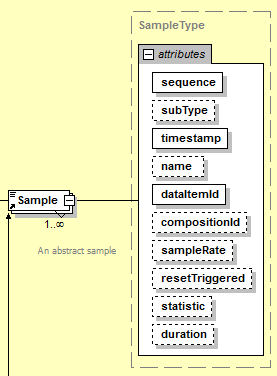
\includegraphics[width=0.5\textwidth]{figures/sample-schema-diagram.png}
  \caption{Sample Schema Diagram}
  \label{fig:sample-schema-diagram}
\end{figure}
\FloatBarrier

\subsubsection{Attributes for Sample}

The \tbl{attributes-for-sample} defines the attributes used to provide additional information for a \gls{sample} XML element.   


\tabulinesep = 5pt
\begin{longtabu} to \textwidth {
    |l|X[3l]|X[0.75l]|}
\caption{Attributes for  Sample} \label{table:attributes-for-sample} \\

\hline
Attribute & Description & Occurrence \\
\hline
\endfirsthead

\hline
\multicolumn{3}{|c|}{Continuation of Table \ref{table:attributes-for-sample}}\\
\hline
Attribute & Description & Occurrence \\
\hline
\endhead
 
\gls{sequence} 
&
A number representing the sequential position of an occurrence of the
\gls{sample} in the data buffer of an \gls{agent}.
\newline \gls{sequence} is a required attribute.
\newline \gls{sequence} \MUST have a value represented as an unsigned 64-bit
value from 1 to $2^{64}-1$.
&
1 \\
\hline

\gls{subtype} 
&
The \gls{subtype} of the \gls{data entity}.
\newline \gls{subtype} is an optional attribute.
\newline \gls{subtype} \MUST match the \gls{subtype} attribute of the \gls{dataitem} element as defined in the \gls{mtconnectdevices} document that the
\gls{sample} element represents. 
&
0..1 \\
\hline

\gls{timestamp} 
&
The most accurate time available to a piece of equipment that represents
the point in time that the data reported for the \gls{sample} was measured.
\newline When the \gls{sample} element represents a \gls{dataitem} element defined in the \gls{mtconnectdevices} document with a \gls{representation} or
\gls{statistic} attribute, \gls{timestamp} \MUST represent the time that the
data collection was completed.
\newline \gls{timestamp} is a required attribute.
&
1 \\
\hline

\gls{name} 
&
The name of the \gls{sample} element.
\newline \gls{name}  is an optional attribute.
\newline \gls{name}  \MUST match the \gls{name}  attribute of the \gls{dataitem} element defined in the \gls{mtconnectdevices} document that the \gls{sample}
element represents.
\newline An \gls{nmtoken} XML type. 
&
0..1 \\
\hline

\gls{dataitemid} 
&
The unique identifier for the \gls{sample} element.
\newline \gls{dataitemid} is a required attribute.
\newline \gls{dataitemid} \MUST match the id attribute of the \gls{dataitem}
element defined in the \gls{mtconnectdevices} document that the
\gls{sample} element represents. 
&
1 \\
\hline

\gls{samplerate} 
&
The rate at which successive samples of the value of a data item are
recorded. \gls{samplerate} is expressed in terms of samples per second.
\newline \gls{samplerate} is an optional attribute.
\newline If the \gls{samplerate} is smaller than one, the number can be represented as a decimal type floating-point number. For example, a rate of 1 per 10 seconds would be 0.1
\newline \gls{samplerate} \MUST be provided when the representation
attribute of the \gls{dataitem} element defined in the
\gls{mtconnectdevices} document that this \gls{sample} element represents
is \gls{timeseries representation}.
\newline For \gls{dataitem} elements where the representation attribute
defined in the \gls{mtconnectdevices} document that this \gls{sample}
element represents is not \gls{timeseries representation}, it \MUST be assumed that the
data reported is represented by a single value and \gls{samplerate} \MUSTNOT be reported in the \gls{mtconnectstreams} document.
&
0..1 \\
\hline

\gls{statistic}
&
The type of statistical calculation defined by the \gls{statistic} attribute
of the \gls{dataitem} element defined in the \gls{mtconnectdevices}
document that this \gls{sample} element represents.
\newline \gls{statistic} is an optional attribute.
&
0..1 \\
\hline

\gls{duration}
&
The time-period over which the data was collected.
\newline \gls{duration} is an optional attribute.
\newline \gls{duration} \MUST be provided when the\gls{statistic} attribute of the \gls{dataitem} element is defined in the \gls{mtconnectdevices} document
that this \gls{sample} element represents.
&
0..1 \\
\hline

\gls{resettriggered}
&
For those \gls{dataitem} elements that report data that may be periodically
reset to an initial value, \gls{resettriggered} identifies when a reported
value has been reset and what has caused that reset to occur.
\newline \gls{resettriggered} is an optional attribute.
\newline \gls{resettriggered} \MUST only be provided for the specific
occurrence of a \gls{data entity} reported in the \gls{mtconnectstreams}
document when the reset occurred and \MUSTNOT be provided for any
other occurrence of the \gls{data entity} reported in a
\gls{mtconnectstreams} document.
&
0..1 \\
\hline

\gls{compositionid}
&
The identifier of the \gls{composition} element defined in the
\gls{mtconnectdevices} document associated with the data reported for
the \gls{sample} element.
\newline \gls{compositionid} is an optional attribute.
&
0..1 \\
\hline

\end{longtabu}

\newpage

\paragraph{duration Attribute for Sample}\mbox{}

\gls{sample} elements that represent the result of a computed value of a statistic \must contain a \gls{duration} attribute.  For these \glspl{data entity}, the \gls{timestamp} associated with the \gls{sample} \must reference the time the data collection was completed.  \gls{timestamp} \MUSTNOT represent any other time associated with the data collection or the calculation of the statistic.  The actual time the interval began can be computed by subtracting the \gls{duration} from the \gls{timestamp}.

Two \gls{sample} elements \may have overlapping time periods when statistics are computed at different frequencies.  For example, there may be two \glspl{data entity} reporting a statistic representing the average value for the readings of the same measured signal calculated over one and five minute intervals.  These \glspl{data entity} can both have the same start time for their calculations (e.g., 05:10:00), but the \gls{timestamp} and \gls{duration} will be 05:11:00 and 60 seconds, respectively, for the \gls{data entity} reporting the one-minute average and 05:15:00 and 300 seconds, respectively, for the \gls{data entity} reporting the five-minute average.  This allows for varying statistical methods to be applied with different interval lengths each having different values for the \gls{timestamp} and \gls{duration} attributes.  

\paragraph{resetTriggered Attribute for Sample}\mbox{}

Some \glspl{data entity} \may have their reported value reset to an initial value.  These reset actions may be based upon a specific elapsed time or may be triggered by a physical or logical reset action that causes the reset to occur.   Examples of \glspl{data entity} that \may have their reported value reset to an initial value are \glspl{data entity} representing a counter, a timer, or a statistic.

\gls{resettriggered} defines the \gls{type} of reset action that caused the value of the reported data to be reset.  The value reported for \gls{resettriggered} \may be defined by the \gls{resettrigger} element for the \gls{data entity} in the \gls{mtconnectdevices} document that this \gls{sample} element represents.  If the \gls{resettrigger} element is not defined in the \gls{mtconnectdevices} document, a \gls{resettriggered} attribute \should be reported in the \gls{mtconnectstreams} document if the \gls{type} of reset action can be determined and reported by the piece of equipment.

\gls{resettriggered} \must only be reported for the first occurrence of a \gls{data entity} after a reset action has occurred and \mustnot be provided for any other occurrence of the \gls{data entity} reported in a \gls{mtconnectstreams} document.  When a reset occurs, the piece of equipment \must report an occurrence of the \gls{data entity} that was reset even if that occurrence of the \gls{data entity} would normally be suppressed based on the filtering criteria established in the \gls{mtconnectdevices} document that this \gls{sample} element represents.

The \tbl{values-for-resettriggered} provides the values that \may be reported for \gls{resettriggered}:    

\tabulinesep = 5pt
\begin{longtabu} to \textwidth {
    |l|X[3l]|}
\caption{Values for resetTriggered} \label{table:values-for-resettriggered} \\

\hline
Value for resetTriggered & Description\\
\hline
\endfirsthead

\hline
\multicolumn{2}{|c|}{Continuation of Table \ref{table:values-for-resettriggered}} \\
\hline
Value for resetTriggered & Description\\
\hline
\endhead
 
\gls{actioncomplete} & 
The value of the \gls{data entity} that is measuring an action or
operation was reset upon completion of that action or
operation. \\ \hline 

\gls{annual} & 
The value of the \gls{data entity} was reset at the end of a 12-month period.\\ \hline 

\gls{day} & 
The value of the \gls{data entity} was reset at the end of a 24-hour
period.\\ \hline 

\gls{maintenance}
& 
The value of the \gls{data entity} was reset upon completion of a maintenance event.
\\ \hline 

\gls{manual value} &
The value of the \gls{data entity} was reset based on a physical reset action. \\ \hline

\gls{month} & 
The value of the \gls{data entity} was reset at the end of a monthly
period. \\ \hline 

\gls{poweron} & 
The value of the \gls{data entity} was reset when power was
applied to the piece of equipment after a planned or unplanned
interruption of power has occurred.\\ \hline 

\gls{shift} & 
The value of the \gls{data entity} was reset at the end of a work
shift.\\ \hline 

\gls{week} & 
The value of the \gls{data entity} was reset at the end of a 7-day
period.\\ \hline 




\end{longtabu}


\subsubsection{Response for SAMPLE category DataItem Elements with a representation Attribute of TIME\_SERIES}
\label{sec:Response for SAMPLE category DataItem Elements with a representation Attribute of TIME_SERIES}

\gls{sample category} category \gls{dataitem} elements defined in the \gls{mtconnectdevices} document with a \gls{representation} attribute of \gls{timeseries representation} \must be represented in the \gls{mtconnectstreams} document as \gls{sample} elements that report data that includes multiple values representing a series of readings of a measured value taken at a specific sample rate.   Such a \gls{dataitem} element can be defined for collecting high frequency readings of a measured value and then providing the entire series of values to a client software application as the data reported for a single \gls{data entity}.  In this case, the \gls{samplecount} and \gls{samplerate} attributes \must be provided. 

\begin{note}
Note: \gls{samplecount} is an attribute that \must only be provided for \gls{sample} elements that represent \gls{sample category} category \gls{dataitem} elements defined in the \gls{mtconnectdevices} document with a \gls{representation} attribute of \gls{timeseries representation}.  

\end{note}

The \gls{cdata} provided for the \gls{data entity} \must be a series of space delimited floating-point numbers.  The number of values \must match the \gls{samplecount}.  

\paragraph{XML Schema Structure for Sample when reporting Time Series Data}\mbox{}

The XML schema in \fig{abstimeseries-schema-diagram}  represents the extended structure of a \gls{sample} XML element that represents a \gls{sample category} category \gls{dataitem} element defined in the \gls{mtconnectdevices} document with a \gls{representation} attribute of \gls{timeseries representation}. 

\begin{figure}[ht]
  \centering
  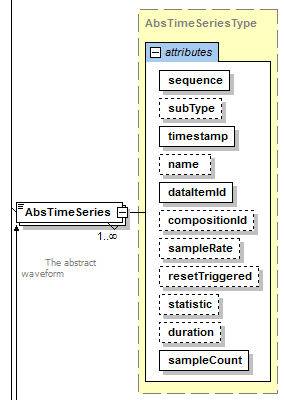
\includegraphics[width=0.5\textwidth]{figures/abstimeseries-schema-diagram.png}
  \caption{AbsTimeSeries Schema Diagram}
  \label{fig:abstimeseries-schema-diagram}
\end{figure}
\FloatBarrier

\begin{note}
Note: The \gls{abstimeseries} element shown in the XML schema is an abstract type element and will be replaced in the \gls{mtconnectstreams} document by the \gls{element name} derived from the \gls{type} attribute defined for the associated \gls{dataitem} element defined in the \gls{mtconnectdevices} document.

\end{note}

\paragraph{Attributes for a Sample when reporting Time Series Data}\mbox{}

\tbl{mtconnect-samplecount-attribute} defines the additional attribute provided for a \gls{sample} XML element that represents a \gls{sample category} category \gls{dataitem} element defined in the \gls{mtconnectdevices} document with a representation attribute of \gls{timeseries representation}. 

\tabulinesep = 5pt
\begin{longtabu} to \textwidth {
    |l|X[3l]|X[0.75l]|}
\caption{MTConnect sampleCount Attribute} \label{table:mtconnect-samplecount-attribute} \\

\hline
Attribute & Description & Occurrence \\
\hline
\endfirsthead

\hline
\multicolumn{3}{|c|}{Continuation of Table \ref{table:mtconnect-samplecount-attribute}}\\
\hline
Attribute & Description & Occurrence \\
\hline
\endhead
 
\gls{samplecount}
&
The number of readings reported in the data returned for the \gls{dataitem}
element defined in the \gls{mtconnectdevices} document that this
\gls{sample} element represents.
\newline \gls{samplecount} is an optional attribute.
\newline \gls{samplecount} \MUST be provided when the representation
attribute of the \gls{dataitem} element is \gls{timeseries representation}.
\newline \gls{samplecount} \MUSTNOT be provided when the
\gls{representation} attribute is defined as \gls{discrete representation} or \gls{value representation}, or
when it is not defined.
&
0..1 \\
\hline

\end{longtabu}


\subsubsection{Response for SAMPLE category DataItem Elements with a representation attribute of DATA_SET}
\label{sec:Response for SAMPLE category DataItem Elements with a representation attribute of DATA_SET}

\gls{sample category} category \gls{dataitem} elements defined in the \gls{mtconnectdevices} document with a \gls{representation} attribute of \gls{dataset} \MUST be represented in the \gls{mtconnectstreams} document as \gls{sample} XML Elements reported as a  \gls{data set} of \glspl{key-value pair}. \gls{dataset} provides the capability to report a set of related data values as a single \gls{data entity}.

The \gls{sample} XML Element acts as a container for \gls{entry} elements to provide a \gls{data set} of \glspl{key-value pair} where each \gls{key model} attribute of the \gls{entry} \MUST be unique and acts as the identity of the \gls{key-value pair}. The CDATA of the \gls{entry} element represents the value portion of the \gls{key-value pair} and has the same constraints as the \gls{data entity} type defined for the \gls{dataitem} \gls{type}.

\paragraph{XML Schema Structure for Sample when reporting Data Set data}\mbox{}
\label{sec:XML Schema Structure for Sample when reporting Data Set data}

\fig{sample-data-set-schema-diagram} represents the XML schema of a \gls{sample} XML element that represents a \gls{sample category} category \gls{dataitem} element defined in the \gls{mtconnectdevices} document with a \gls{representation} attribute of \gls{dataset}.

\begin{figure}[ht]
  \centering
  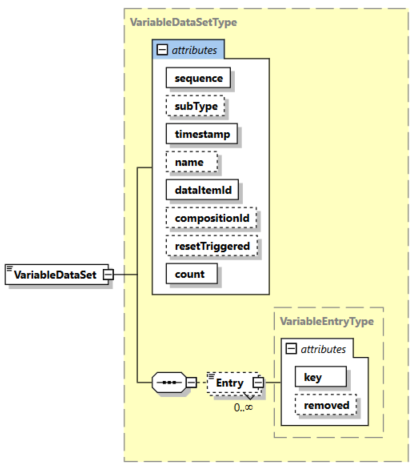
\includegraphics[width=0.7\textwidth]{figures/sample-data-set-schema-diagram.png}
  \caption{Sample Data Set Schema Diagram}
  \label{fig:sample-data-set-schema-diagram}
\end{figure}
\FloatBarrier

\paragraph{Attributes for Sample when reporting Data Set data}\mbox{}
\label{sec:Attributes for Sample when reporting Data Set data}

\tbl{attributes-for-dataset} defines the additional attribute provided for a \gls{sample} XML element that represents a \gls{sample category} category \gls{dataitem} element defined in the \gls{mtconnectdevices} document with a \gls{representation} attribute of \gls{dataset}.


\begin{longtabu} to \textwidth{|l|X[3l]|l|}
\caption{Attributes for DataSet} \label{table:attributes-for-dataset} \\

\hline
Attribute & Description & Occurrence \\
\hline
\endfirsthead

\hline
\multicolumn{3}{|c|}{Continuation of Table \ref{table:attributes-for-dataset}}\\
\hline
Attribute & Description & Occurrence \\
\hline
\endhead
 




\gls{count model}
&
Represents the number of \glspl{key-value pair} represented as \gls{entry} elements as the contents of the \gls{sample} element.
\newline \gls{count model} \MUST be provided when the \gls{representation} attribute of the \gls{dataitem} element is \gls{dataset}.
\newline \gls{count model} \MUSTNOT be provided when the \gls{representation} attribute is defined as \gls{discrete representation}, \gls{timeseries representation}, or \gls{value representation}, or when it is not defined.
&
0..1 \\
\hline\end{longtabu}

\paragraph{Elements for Sample when reporting Data Set data}\mbox{}
\label{sec:Elements for Sample when reporting Data Set data}

\tbl{elements-for-dataset} defines the elements provided for a \gls{sample} XML element that represents a \gls{sample category} category \gls{dataitem} element defined in the \gls{mtconnectdevices} document with a \gls{representation} attribute of \gls{dataset}. \gls{entry} is the only child element that \MAY be associated with a \gls{data entity} with a \gls{representation} attribute of \gls{dataset}. Each \gls{entry} element represents a unique \gls{key-value pair}. 


\begin{longtabu} to \textwidth{|l|X[3l]|l|}
\caption{Elements for DataSet} \label{table:elements-for-dataset} \\

\hline
Element & Description & Occurrence \\
\hline
\endfirsthead

\hline
\multicolumn{3}{|c|}{Continuation of Table \ref{table:elements-for-dataset}}\\
\hline
Element & Description & Occurrence \\
\hline
\endhead
 




\gls{entry}
&
A XML element representing a \gls{key-value pair} published as part of a \gls{data set}.
&
0..* \\
\hline\end{longtabu}

\subparagraph{XML Schema Structure for Entry Element for a Data Entity}\mbox{}
\label{sec:XML Schema Structure for Entry Element for a Data Entity}

\fig{entry-element-schema-diagram} represents the XML Schema structure for a \gls{entry} XML element that represents the information published for a \gls{key-value pair}. Any number of \gls{entry} elements \MAY be provided for a \gls{data entity} defined with a \gls{representation} attribute of \gls{dataset}. 

\begin{figure}[ht]
  \centering
  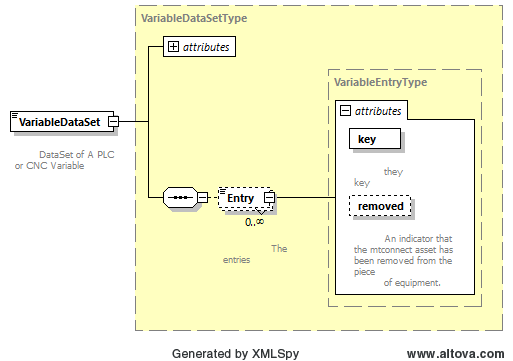
\includegraphics[width=0.8\textwidth]{figures/entry-element-schema-diagram.png}
  \caption{Entry Element Schema Diagram}
  \label{fig:entry-element-schema-diagram}
\end{figure}
\FloatBarrier

\begin{note}
Note: The \cfont{VariableDataSet} element shown in the XML schema is an example that illustrates the schema for a \gls{data entity} element and its associated \gls{entry} elements representing a \gls{data set}.

\end{note}

The following example demonstrates how multiple \glspl{key-value pair}, each defined by an \gls{entry} element, are structured in a \gls{mtconnectstreams} document.
\begin{lstlisting}[firstnumber=1,escapechar=|,%
    caption={Example of multiple key-value pairs Reported for a Data Entity},label={lst:example-of-multiple-key-value-pairs-reported-for-a-data-entity}]
  <VariableDataSet timestamp="..." sequence="..." count="2">
    <Entry key="a101">100.21</Entry>
    <Entry key="a102">609</Entry>
    <Entry key="a103" removed="true" />
  </VariableDataSet>
\end{lstlisting}

\subparagraph{Attributes for Entry Element for a Data Entity}\mbox{}
\label{sec:Attributes for Entry Element for a Data Entity}

The \tbl{attributes-for-entry} defines the attributes provided for a \gls{entry} XML element. 


\begin{longtabu} to \textwidth{|l|X[3l]|l|}
\caption{Attributes for Entry} \label{table:attributes-for-entry} \\

\hline
Attribute & Description & Occurrence \\
\hline
\endfirsthead

\hline
\multicolumn{3}{|c|}{Continuation of Table \ref{table:attributes-for-entry}}\\
\hline
Attribute & Description & Occurrence \\
\hline
\endhead
 




\gls{key model}
&
A unique identifier for each \gls{key-value pair}.
\newline The value provided for \gls{key model} \MUST be unique in any given set of \gls{entry} elements.
\newline The value provided for \gls{key model} \MUST be a XML NMTOKEN type.
&
1 \\
\hline

\gls{removed}
&
A indicator defining whether a specific \gls{key-value pair} has been removed from the set of \glspl{key-value pair} associated with this \gls{data set}.
\newline \gls{removed} is an XML Boolean type that \MUST have a value of \gls{true removed} or \gls{false removed}.
\newline \gls{true removed} indicates that the \gls{key-value pair} has been removed from the \gls{data set}.
\newline \gls{false removed} indicates that the \gls{key-value pair} has not been removed from the \gls{data set}.
\newline If not specified, the default value for \gls{removed} is \gls{false removed}
&
0..1 \\
\hline\end{longtabu}


\subsubsection{Valid Data Values for Sample}

All \gls{sample} elements reported in an \gls{mtconnectstreams} XML document \must provide a value in the \gls{cdata} of the \gls{data entity}.

The value returned in the \gls{cdata} \must be reported as either a \gls{valid data value} representing the information reported from a piece of equipment or \gls{unavailable value} when a \gls{valid data value} cannot be determined.

The \gls{valid data value} reported for a \gls{sample} represents the reading of the value of a continuously variable or analog data source.

The \gls{representation} attribute for a \gls{sample category} category \gls{dataitem} element defined in the \gls{mtconnectdevices} document specifies how an \gls{agent} \must record instances of the data associated with that data item and how often that data \must be reported as a \gls{sample} element in the \gls{mtconnectstreams} document.

The data reported for a \gls{sample} element associated with a \gls{sample category} category \gls{dataitem} element with a \gls{representation} of \gls{value representation} can be measured at any point-in-time and \must always produce a result with a single data value.  

\begin{note}
Note: If a \gls{representation} attribute is not specified in the \gls{mtconnectdevices} document for a \gls{dataitem} element, it \must be assumed that the data reported in the \gls{mtconnectstreams} document for the \gls{data entity} has a \gls{representation} type of \gls{value representation}.

\end{note}

In the case of a \gls{sample} element associated with a \gls{sample category} category \gls{dataitem} element with a \gls{representation} attribute of \gls{timeseries representation}, the data provided \must be a series of data values representing multiple sequential samples of the measured value that will be provided only at the end of the completion of a sampling period.   (See Section \sect{Response for SAMPLE category DataItem Elements with a representation Attribute of TIME_SERIES} for more information on \gls{timeseries representation} type data).

In the case of a \gls{sample} element associated with a \gls{sample category} category \gls{dataitem} element with a \gls{representation} attribute of \gls{dataset}, the data reported for each \gls{key-value pair} \MUST be provided in the same \glspl{valid data value} and units as specified by the \gls{type} attribute for the \gls{dataitem} element.

When an \gls{agent} responds to a \gls{current request}, the information returned in the \gls{mtconnectstreams} document for a \gls{data entity} defined to represent a \gls{data set} \MUST include the full set of \glspl{key-value pair} that are valid for that \gls{data entity}. If the \gls{current request} includes an \gls{at query} \textit{query parameter}, the \gls{agent} \MUST provide the set of \glspl{key-value pair} that are valid at the specified \gls{sequence number}.

When an \gls{agent} responds to a \gls{sample request}, the information returned in the \gls{mtconnectstreams} document for a \gls{data entity} defined to represent a \gls{data set} \MUST include only those \glspl{key-value pair} that are valid for the \gls{data entity} at each \gls{sequence number}. 

Data values provided for a \gls{sample} \must always be a floating-point number.   In the MTConnect Standard, floating-point numbers are defined as XML xs:float \gls{type} numbers as defined by W3C.  Any of the following number formats are valid XML floating \gls{type} numbers: 1267.43233E12, -1E4, 12.78e-2, 12, 137.2847, 0, and INF.  

\begin{note}
Note: For some \gls{sample} elements, the \gls{valid data value} \may be restricted to specific formats.  See Section 6.1 of this document for a description of any restrictions of the acceptable format for \gls{valid data value}.

\end{note}

For \gls{sample} elements, a client software application can determine the appropriate accuracy of the value reported for the \gls{data entity} by applying the significantDigits attribute defined for the corresponding \gls{dataitem} element defined in the \gls{mtconnectdevices} document.

The \gls{valid data value} reported as \gls{cdata} for a \gls{sample} element \must be formatted as part of the content between the element tags in the XML element representing that \gls{data entity}.  As an example, a \glselementname{position sample} is formatted as shown in \lst{example-of-sample-position}.

\begin{lstlisting}[firstnumber=1,escapechar=|,%
    caption={Example showing CDATA of a DataItem Element},label={lst:example-of-sample-position}]
<Position sequence="112" name="Xabs"
    timestamp="2016-07-28T02:06:01.364428Z" 
    dataItemId="10">123.3333</Position>
\end{lstlisting}

In this example, the 123.3333 is the \gls{cdata} for \glselementname{position sample}.   All \gls{cdata} in a \gls{sample} element is typed, which means that the value reported for the \gls{data entity} \must be formatted as defined in Section 6.1 for each \gls{data entity} so that it can be validated.

\subsubsection{Unavailability of Valid Data Values for Sample}

If an \gls{agent} cannot determine a \gls{valid data value} for a \gls{sample} element, the value returned for the \gls{cdata} for the \gls{data entity} \must be reported as \gls{unavailable value}.

\lst{example-of-cdata-unavailable} demonstrates how an \gls{agent} reports the value for a \gls{sample} in the \gls{cdata} when it is unable to determine a \gls{valid data value}:  


\begin{lstlisting}[firstnumber=1,escapechar=|,%
    caption={Example of CDATA when Data Entity is  UNAVAILABLE},label={lst:example-of-cdata-unavailable}]
<Samples>
  <PathPosition dataItemId="p2"
      timestamp="2009-03-04T19:45:50.458305"
      subType="ACTUAL" name="Zact"
      sequence="15065113">UNAVAILABLE</PathPosition>
  <Temperature dataItemId="t6"
      timestamp="2009-03-04T19:45:50.458305" name="temp" 
      sequence="150651134">UNAVAILABLE</Temperature>
</Samples>
\end{lstlisting}

\subsection{Events Container}

\gls{events} is a XML container type element.  \gls{events} organizes the \glspl{data entity} returned in the \gls{mtconnectstreams} XML document for those \gls{dataitem} elements defined with a \gls{category} attribute of \gls{event category} in the \gls{mtconnectdevices} document.

A separate \gls{events} container will be provided for the data returned for the \gls{dataitem} elements associated with each \gls{structural element} of a piece of equipment defined in the \gls{mtconnectdevices} document.


\tabulinesep = 5pt
\begin{longtabu} to \textwidth {
    |l|X[3l]|X[0.75l]|}
\caption{MTConnect Event Element} \label{table:mtconnect-events-element} \\

\hline
Element & Description & Occurrence \\
\hline
\endfirsthead

\hline
\multicolumn{3}{|c|}{Continuation of Table \ref{table:mtconnect-events-element}}\\
\hline
Element & Description & Occurrence \\
\hline
\endhead
 
\gls{events}
&
\glsentrydesc{events} 
\newline A separate \gls{events} container \MUST be provided for each
\gls{componentstream} element for which data is returned for a \gls{dataitem}
element defined in the \gls{mtconnectdevices} document with a category
attribute of \gls{event category}.
\newline If provided in the document, an \gls{events} XML container \MUST contain at least one \gls{event} element.
&
0..1 \\
\hline

\end{longtabu}


\subsection{Event Data Entities}

An \gls{event} XML element provides the information and data provided from a piece of equipment for those \gls{dataitem} elements defined with a \gls{category} attribute of \gls{event category} in the \gls{mtconnectdevices} document.

\gls{event} is an abstract \gls{type} XML element and will never appear directly in the \gls{mtconnectstreams} XML document.  As an abstract \gls{type} XML element, \gls{event} will be replaced in the XML document by a specific \gls{type} of \gls{event} specified by the \gls{element name} for that \gls{data entity}.  The different \glspl{type} of \gls{event} elements are defined in \sect{Event Element Names}.  Examples of XML elements representing \gls{event} include \glselementname{block event} and \glselementname{execution event}.

\gls{event} is similar to \gls{sample}, but its value can change with unpredictable frequency.  \gls{events} do not report intermediate values.  As an example, when \glselementname{availability event} transitions from \gls{unavailable value} to \gls{available value}, there is no intermediate state that can be inferred.

\gls{event} elements \may report data values defined by a controlled vocabulary as specified in \sect{Event Element Names}, by numeric values, or by a character string representing text or a message provided by the piece of equipment. 


\tabulinesep = 5pt
\begin{longtabu} to \textwidth {
    |l|X[3l]|X[0.75l]|}
\caption{MTConnect Event Element} \label{table:mtconnect-event-element} \\

\hline
Element & Description & Occurrence \\
\hline
\endfirsthead

\hline
\multicolumn{3}{|c|}{Continuation of Table \ref{table:mtconnect-event-element}}\\
\hline
Element & Description & Occurrence \\
\hline
\endhead
 
\gls{event}
&
\glsentrydesc{event} 
\newline \gls{event} is an abstract type XML element. It is replaced in the
\gls{mtconnectstreams} document by a specific type of \gls{event} element.
\newline There \MAY be multiple types of \gls{event} elements in a \glspl{event} container.
&
1..* \\
\hline

\end{longtabu}


\subsubsection{XML Schema Structure for Event}

The XML schema in \fig{event-schema-diagram} represents the structure of an \gls{event} XML element showing the attributes defined for \gls{event} elements.

\begin{figure}[ht]
  \centering
  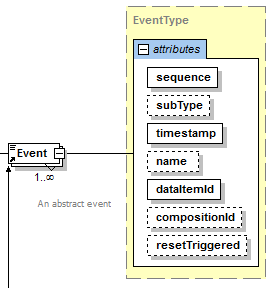
\includegraphics[width=0.5\textwidth]{figures/event-schema-diagram.png}
  \caption{Event Schema Diagram}
  \label{fig:event-schema-diagram}
\end{figure}

\FloatBarrier

\subsubsection{Attributes for Event}

\tbl{attributes-for-event} defines the attributes that \may be used to provide additional information for an \gls{event} XML element.


\tabulinesep = 5pt
\begin{longtabu} to \textwidth {
    |l|X[3l]|X[0.75l]|}
\caption{Attributes for Event} \label{table:attributes-for-event} \\

\hline
Attribute & Description & Occurrence \\
\hline
\endfirsthead

\hline
\multicolumn{3}{|c|}{Continuation of Table \ref{table:attributes-for-event}}\\
\hline
Attribute & Description & Occurrence \\
\hline
\endhead
 
\gls{sequence} 
&
A number representing the sequential position of an occurrence of the
\gls{event} in the data buffer of an \gls{agent}.
\newline \gls{sequence} is a required attribute.
\newline \gls{sequence} \MUST have a value represented as an unsigned 64-bit
value from 1 to $2^{64}-1$.
&
1 \\
\hline

\gls{subtype} 
&
The \gls{subtype} of the \gls{data entity}.
\newline \gls{subtype} is an optional attribute.
\newline \gls{subtype} \MUST match the \gls{subtype} attribute of the \gls{dataitem} element as defined in the \gls{mtconnectdevices} document that the
\gls{event} element represents. 
&
0..1 \\
\hline

\gls{timestamp} 
&
The most accurate time available to a piece of equipment that represents
the point in time that the data reported for the \gls{event} was measured.
\newline \gls{timestamp} is a required attribute.
&
1 \\
\hline

\gls{name} 
&
The name of the \gls{event} element.
\newline \gls{name}  is an optional attribute.
\newline \gls{name}  \MUST match the \gls{name}  attribute of the \gls{dataitem} element defined in the \gls{mtconnectdevices} document that the \gls{event}
element represents.
\newline An \gls{nmtoken} XML type. 
&
0..1 \\
\hline

\gls{dataitemid} 
&
The unique identifier for the\gls{event} element.
\newline \gls{dataitemid} is a required attribute.
\newline \gls{dataitemid} \MUST match the id attribute of the \gls{dataitem}
element defined in the \gls{mtconnectdevices} document that the
\gls{event} element represents. 
&
1 \\
\hline

\gls{resettriggered}
&
For those \gls{dataitem} elements that report data that may be periodically
reset to an initial value, \gls{resettriggered} identifies when a reported
value has been reset and what has caused that reset to occur.
\newline \gls{resettriggered} is an optional attribute.
\newline \gls{resettriggered} \MUST only be provided for the specific
occurrence of a \gls{data entity} reported in the \gls{mtconnectstreams}
document when the reset occurred and \MUSTNOT be provided for any
other occurrence of the \gls{data entity} reported in a
\gls{mtconnectstreams} document.
&
0..1 \\
\hline

\gls{compositionid}
&
The identifier of the \gls{composition} element defined in the
\gls{mtconnectdevices} document associated with the data reported for
the \gls{event} element.
\newline \gls{compositionid} is an optional attribute.
&
0..1 \\
\hline

\end{longtabu}

  

\subsubsection{Response for EVENT category DataItem Elements with a representation attribute of DATA_SET}
\label{sec:Response for EVENT category DataItem Elements with a representation attribute of DATA_SET}

The behavior of \gls{event category} category \gls{dataitem} elements defined in the \gls{mtconnectdevices} document with a \gls{representation} attribute of \gls{dataset} function exactly the same as \gls{sample category} category \gls{dataitem} elements with a \gls{representation} attribute of \gls{dataset}. Refer to \sect{Response for SAMPLE category DataItem Elements with a representation attribute of DATA_SET} for details on \gls{dataitem} elements with a \gls{representation} attribute of \gls{dataset}.  


\subsubsection{Valid Data Values for Event}

\gls{event} elements reported in an \gls{mtconnectstreams} XML document \must provide a value in the \gls{cdata} of the \gls{data entity}.

The value reported in the \gls{cdata} \must be reported as either a \gls{valid data value} representing the information reported from a piece of equipment or \gls{unavailable value} when a \gls{valid data value} cannot be determined.

The \gls{valid data value} reported for an \gls{event} represents a distinct piece of information provided from a piece of equipment.  Unlike \gls{sample}, \gls{event} does not report intermediate values that vary over time.  \gls{event} reports information that, when provided at any specific point in time, represents the current state of the piece of equipment.

The \gls{representation} attribute for an \gls{event category} category data item defined in the \gls{mtconnectdevices} document specifies how an \gls{agent} \must record instances of data associated with that data item and how that data \must be reported as an \gls{event} element in the \gls{mtconnectstreams} document.

The data reported for an \gls{event} element associated with an \gls{event category} category data item with a \gls{representation} attribute of \gls{value representation} \must be either an integer, a floating-point number, a descriptive value (text string) representing one of two or more state values defined for that data item, or a text string representing a message.

If a \gls{representation} attribute is not specified for a data item in an \gls{mtconnectdevices} document, the designation for the \gls{representation} attribute \must be interpreted as \gls{value representation}.

In the case of an \gls{event} element associated with a \gls{event category} category \gls{dataitem} element with a \gls{representation} attribute of \gls{dataset}, the data reported for each \gls{key-value pair} \MUST be provided in the same \glspl{valid data value} and units as specified by the \gls{type} attribute for the \gls{dataitem} element.

When an \gls{agent} responds to a \gls{current request}, the information returned in the \gls{mtconnectstreams} document for a \gls{data entity} defined to represent a \gls{data set} \MUST include the full set of \glspl{key-value pair} that are valid for that \gls{data entity}. If the \gls{current request} includes an \gls{at query} \textit{query parameter}, the \gls{agent} \MUST provide the set of \glspl{key-value pair} that are valid at the specified \gls{sequence number}.

When an \gls{agent} responds to a \gls{sample request}, the information returned in the \gls{mtconnectstreams} document for a \gls{data entity} defined to represent a \gls{data set} \MUST include only those \glspl{key-value pair} that are valid for the \gls{data entity} at each \gls{sequence number}
The \gls{valid data value} reported as CDATA for an \gls{event} element \must be formatted as part of the content between the element tags in the XML element representing that \gls{data entity}.  As an example, \gls{event} elements are formatted as shown in \lst{example-of-event-element}:

\begin{lstlisting}[firstnumber=1,escapechar=|,%
    caption={Example of Event Element},label={lst:example-of-event-element}]
<PartCount dataItemId="pc4" 
    timestamp="2009-02-26T02:02:36.48303"
    name="pcount" sequence="185">238</PartCount>
<ControllerMode dataItemId="p3" 
    timestamp="2009-02-26T02:02:35.716224"
    name="mode" sequence="192">AUTOMATIC</ControllerMode>
    <Block dataItemId="cn2" name="block" sequence="206"
        timestamp="2009-02-26T02:02:37.394055">G0Z1</Block>
\end{lstlisting}


In these examples, \cfont{238} is the \gls{cdata} for \glselementname{partcount} and is a numeric value; \gls{automatic value} is the \gls{cdata} for the \glselementname{controllermode event} and is a descriptive value representing a state for the \gls{data entity}; and \cfont{G0Z1} is a text string representing a message describing the program code associated with the \glselementname{block event} \gls{data entity}. 

\subsubsection{Unavailability of Valid Data Value for Event}

If an \gls{agent} cannot determine a \gls{valid data value} for an \gls{event} element, the value returned for the \gls{cdata} for the \gls{data entity} \must be reported as \gls{unavailable value}.

The example in \lst{example-of-event-element-unavailable} demonstrates how an \gls{agent} reports the value for an \gls{event} in the \gls{cdata} when it is unable to determine a \gls{valid data value}:  

\begin{lstlisting}[firstnumber=1,escapechar=|,%
    caption={Example of Event Element when data value is UNAVAILABLE},label={lst:example-of-event-element-unavailable}]
<Events>
  <ControllerMode dataItemId="p3" 
      timestamp="2009-02-26T02:02:35.716224" name="mode"
      sequence="182">UNAVAILABLE</ControllerMode>
</Events>
\end{lstlisting}


\subsection{Condition Container}

\gls{conditions} is a XML container type element.  \gls{conditions} organizes the \glspl{data entity} returned in the \gls{mtconnectstreams} XML document for those \gls{dataitem} elements defined with a \gls{category} attribute of \gls{condition category} in the \gls{mtconnectdevices} document.

A separate \gls{conditions} container will be provided for the data returned for the \gls{dataitem} elements associated with each \gls{structural element} of a piece of equipment defined in the \gls{mtconnectdevices} document.

\tabulinesep = 5pt
\begin{longtabu} to \textwidth {
    |l|X[3l]|X[0.75l]|}
\caption{MTConnect Condition Element Container} \label{table:mtconnect-conditions-element-container} \\

\hline
Element & Description & Occurrence \\
\hline
\endfirsthead

\hline
\multicolumn{3}{|c|}{Continuation of Table \ref{table:mtconnect-conditions-element-container}}\\
\hline
Element & Description & Occurrence \\
\hline
\endhead
 
\gls{conditions}
&
\glsentrydesc{conditions} 
\newline A separate \gls{conditions} container \MUST be provided for each
\gls{componentstream} element for which data is returned for a \gls{dataitem}
element defined in the \gls{mtconnectdevices} document with a category attribute of \gls{condition category}.
\newline If provided in the document, a \gls{conditions} XML container \MUST contain at least one \gls{condition} element.
&
0..1 \\
\hline

\end{longtabu}


\subsection{Condition Data Entity}\label{sec:Condition Data Entity}

A \gls{condition} XML element provides the information and data provided from a piece of equipment for those \gls{dataitem} elements defined with a \gls{category} attribute of \gls{condition category} in the \gls{mtconnectdevices} document.  

\gls{condition} provides information reported by a piece of equipment describing its health and ability to function.

\gls{condition} is an abstract type XML element and will never appear directly in the \gls{mtconnectstreams} XML document.  As an abstract type XML element, \gls{condition} will be replaced in the XML document by a \gls{data entity} representing the \gls{condition category} category \gls{dataitem} element defined in the \gls{mtconnectdevices} document that this \gls{condition} element represents.

The \glspl{data entity} represented by \gls{condition} are structured differently than the \glspl{data entity} representing \gls{sample} and \gls{event}.   The \gls{element name} for each \gls{condition} element reported in the \gls{mtconnectstreams} document defines the \gls{fault state} of the \gls{data entity}.  A \gls{condition} element is identified by the \gls{structural element} to which it is associated, along with the \gls{type} and \gls{dataitemid} defined for the element.  \sect{Types of Condition Elements} provides details on the different \glspl{type} of \gls{condition} elements.

\tabulinesep = 5pt
\begin{longtabu} to \textwidth {
    |l|X[3l]|X[0.75l]|}
\caption{MTConnect Condition Element} \label{table:mtconnect-condition-element} \\

\hline
Element & Description & Occurrence \\
\hline
\endfirsthead

\hline
\multicolumn{3}{|c|}{Continuation of Table \ref{table:mtconnect-condition-element}}\\
\hline
Element & Description & Occurrence \\
\hline
\endhead
 
\gls{condition}
&
\glsentrydesc{condition} 
\newline \gls{condition} is an abstract type XML element. It is replaced in the
\gls{mtconnectstreams} document by a specific type of \gls{condition} element.
\newline There \MAY be multiple types of \gls{condition} elements in a \glspl{condition} container.
&
1..* \\
\hline

\end{longtabu}


\gls{condition category} type \gls{dataitem} elements defined in the \gls{mtconnectdevices} document \may report multiple simultaneous \glspl{fault state} in the \gls{mtconnectstreams} document.  This is unlike a \gls{sample category} or \gls{event category} \gls{dataitem} element that can only report a single occurrence of a \gls{sample} or \gls{event} element in the \gls{mtconnectstreams} document at any one point in time.

For example, a controller on a piece of equipment may detect and report multiple format errors in a motion program.   Each error represents a separate \gls{fault state} from the controller.   Each \gls{fault state} is represented as a separate \gls{condition} element in the \gls{mtconnectstreams} document since each \gls{fault state} \must be identified and tracked individually in the document.

\subsubsection{Element Names for Condition}\label{sec:Element Names for Condition}

\gls{condition} elements are reported differently from other \gls{data entity} \glspl{type}.  The \gls{element name} reported for a \gls{condition} element represents the \gls{fault state} (\gls{normal}, \gls{warning}, or \gls{fault}) associated with each \gls{condition}.

Examples of XML elements representing \gls{condition} elements for each of the possible \glspl{fault state} are shown in \lst{example-of-condition-element-fault-states}:

\begin{lstlisting}[firstnumber=1,escapechar=|,%
    caption={Example of Condition Element Fault States},label={lst:example-of-condition-element-fault-states}]
<Normal type="MOTION_PROGRAM" dataItemId="cc2" sequence="25"
    timestamp="2010-04-06T06:19:35.153141"</Normal>
<Fault type="COMMUNICATIONS" dataItemId="cc1" sequence="26"
    nativeCode="IO1231" timestamp="2010-04-
    06T06:19:35.153141">Communications error</Fault>
<Warning type="LOGIC_PROGRAM" dataItemId="pm6" sequence="32"
    timestamp="2010-04-06T06:19:35.153141"<Warning/>
\end{lstlisting}

\subsubsection{XML Schema Structure for Condition}

The XML schema in \fig{condition-schema-diagram} represents the structure of a \gls{condition} XML element showing the attributes defined for \gls{condition} elements.

\begin{figure}[ht]
  \centering
  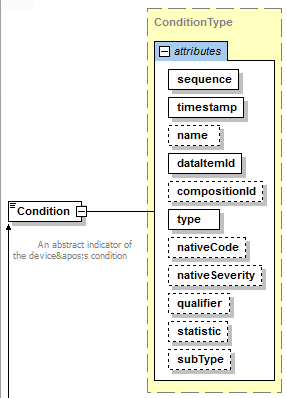
\includegraphics[width=0.6\textwidth]{figures/condition-schema-diagram.png}
  \caption{Condition Schema Diagram}
  \label{fig:condition-schema-diagram}
\end{figure}
\FloatBarrier

\subsubsection{Attributes for Condition}

\tbl{attributes-for-condition} defines the attributes used to provide additional information for a \gls{condition} XML element.


\tabulinesep = 5pt
\begin{longtabu} to \textwidth {
    |l|X[3l]|X[0.75l]|}
\caption{Attributes for Condition} \label{table:attributes-for-condition} \\

\hline
Attribute & Description & Occurrence \\
\hline
\endfirsthead

\hline
\multicolumn{3}{|c|}{Continuation of Table \ref{table:attributes-for-condition}}\\
\hline
Attribute & Description & Occurrence \\
\hline
\endhead
 
\gls{sequence} 
&
A number representing the sequential position of an occurrence of the
\gls{condition} in the data buffer of an MTConnect Agent.
\newline \gls{sequence} is a required attribute.
\newline \gls{sequence} \MUST have a value represented as an unsigned 64-bit value from 1 to $2^{64}-1$.
&
1 \\
\hline

\gls{timestamp} 
&
The most accurate time available to a piece of equipment that represents the point in time that the data reported for the \gls{condition} was measured.
\newline \gls{timestamp} is a required attribute.
&
1 \\
\hline

\gls{name} 
&
The name of the \gls{condition} element.
\newline \gls{name}  is an optional attribute.
\newline \gls{name}  \MUST match the \gls{name}  attribute of the \gls{dataitem} element defined in the \gls{mtconnectdevices} document that the \gls{condition}
element represents.
\newline An \gls{nmtoken} XML type. 
&
0..1 \\
\hline

\gls{dataitemid} 
&
The unique identifier for the\gls{condition} element.
\newline \gls{dataitemid} is a required attribute.
\newline \gls{dataitemid} \MUST match the id attribute of the \gls{dataitem}
element defined in the \gls{mtconnectdevices} document that the
\gls{condition} element represents. 
&
1 \\
\hline

\gls{type} 
&
An identifier of the \gls{type} of fault represented by the \gls{condition} element.
\newline \gls{type} is a required attribute.
\newline \gls{type} \MUST match the \gls{type} attribute of the \gls{dataitem} element defined in the \gls{mtconnectdevices} document that this \gls{condition} element represents. 
&
1 \\
\hline

\gls{nativecode}
&
The native code (usually an alpha-numeric value) generated by the
controller of a piece of equipment providing a reference identifier for a \gls{condition}.
\newline \gls{nativecode} is an optional attribute.
\newline This is the same information an operator or maintenance personnel may see as a reference code designating a specific fault code provided by the piece of equipment. 
&
0..1 \\
\hline

\gls{nativeseverity}
&
If the piece of equipment designates a severity level to a fault,
\gls{nativeseverity} reports that severity information to a client
software application.
\newline \gls{nativeseverity} is an optional attribute.
&
0..1 \\
\hline

\gls{qualifier}
&
\gls{qualifier} provides additional information regarding a \gls{fault state} associated with the measured value of a process variable.
\newline \gls{qualifier} is an optional attribute.
\newline \gls{qualifier} defines whether the \gls{fault state} represented by the \gls{condition} indicates a measured value that is above or below an expected value of a process variable.
\newline If the \gls{fault state} represents a measured value that is greater than the expected value for the process variable, \gls{qualifier} \MUST report a value of \gls{high}.
\newline If the \gls{fault state} represents a measured value that is less than the expected value for the process variable, \gls{qualifier} \MUST report a value of \gls{low}. 
&
0..1 \\
\hline

\gls{statistic}
&
\gls{statistic} provides additional information describing the meaning of the \gls{condition} element.
\newline \gls{statistic} is an optional attribute.
\newline \gls{statistic} \MUST match the \gls{statistic} attribute of the \gls{dataitem} element defined in the \gls{mtconnectdevices} document that this \gls{condition} element represents. 
&
0..1 \\
\hline

\gls{subtype} 
&
\gls{subtype} provides additional information describing the meaning of the \gls{condition} element.
\newline \gls{subtype} is an optional attribute.
\newline \gls{subtype} \MUST match the \gls{subtype} attribute of the \gls{dataitem} element defined in the \gls{mtconnectdevices} document that this \gls{condition} element represents. 
&
0..1 \\
\hline

\gls{compositionid}
&
The identifier of the \gls{composition} element defined in the
\gls{mtconnectdevices} document associated with the data reported for the \gls{condition} element.
\newline \gls{compositionid} is an optional attribute.
&
0..1 \\
\hline

\gls{xs:lang} 
&
An optional attribute that specifies the language of the \gls{cdata} returned for the \gls{condition}.
\newline Refer to IETF RFC 4646 (http://www.ietf.org/rfc/rfc4646.txt) or successor for a full definition of the values for this attribute.
\newline \gls{xs:lang} does not appear in the schema diagram.
&
0..1 \\
\hline

\end{longtabu}

\paragraph{qualifier Attribute for Condition}\mbox{}

Many \gls{condition} elements report the \gls{fault state} associated with the measured value of a process variable.

\gls{qualifier} provides an indication whether the measured value is above or below an expected value of a process variable.

As an example, a \gls{condition} element with a \gls{type} attribute of \gls{amperage sample} may differentiate between a higher than expected amperage and a lower than expected amperage by using the \gls{qualifier} attribute.

When a \gls{qualifier} of either \gls{high} or \gls{low} is used with \gls{fault} and \gls{warning}, the \glspl{fault state} can be differentiated as follows:

\quad \gls{fault},\gls{low}

\quad \gls{warning},\gls{low}

\quad \gls{normal}

\quad \gls{warning},\gls{high}

\quad \gls{fault},\gls{high}
     
\lst{example-of-condition-using-qualifier} is an example of an XML element representing \gls{condition} using \gls{qualifier}:

\begin{lstlisting}[firstnumber=1,escapechar=|,%
    caption={Example of a Condition Element using qualifier},label={lst:example-of-condition-using-qualifier}]
<Warning type="FILL_LEVEL" dataItemId="pm6" 
    qualifier="HIGH" sequence="32" 
    timestamp="2009-11-13T08:32:18">...</Warning>
\end{lstlisting}

\subsubsection{Valid Data Value for Condition}

\gls{condition} elements reported in an \gls{mtconnectstreams} XML document \may provide a value in the \gls{cdata} of the \gls{data entity} when additional information regarding the \gls{fault state} is available.

A \gls{valid data value} for the \gls{cdata} included in a \gls{condition} element \may be any text string.   A \gls{valid data value} is not required to be reported for a \gls{condition} category \gls{data entity}.  The \gls{fault state} and the attributes provided in a \gls{condition} element \may be sufficient to fully describe the \gls{data entity}.

The \gls{valid data value} reported as \gls{cdata} for a \gls{condition} element \must be formatted as part of the content between the element tags in the XML element representing that \gls{data entity}.  As an example, \gls{condition} elements are formatted as shown in \lst{example-of-cdata-for-condition}:

\begin{lstlisting}[firstnumber=1,escapechar=|,%
    caption={Example of CDATA for Condition},label={lst:example-of-cdata-for-condition}]
<Warning type="FILL_LEVEL" dataItemId="pm6" 
    qualifier="HIGH" sequence="32" timestamp=
    "2009-11-13T08:32:18">Fill Level on Tank
    #12 is reaching a high level</Warning>
\end{lstlisting}

In this example, the “Fill Level on Tank \#12 is reaching a high level" is the \gls{cdata} for the \gls{data entity}.

\subsection{Unavailability of Fault State for Condition}\label{sec:Unavailability of Fault State for Condition}

When an \gls{agent} cannot determine a valid \gls{fault state} for a \gls{condition} element, it \must report the \gls{element name} for the \gls{data entity} as Unavailable.

\lst{example-of-condition-when-fault-state-is-unavailable} demonstrates how an \gls{agent} reports a \gls{condition} category \gls{data entity} when it is unable to determine a valid \gls{fault state}:

\begin{lstlisting}[firstnumber=1,escapechar=|,%
    caption={Example of Condition when Fault State is UNAVAILABLE},label={lst:example-of-condition-when-fault-state-is-unavailable}]
<Unavailable type="MOTION_PROGRAM" dataItemId="cc2" 
    sequence="25" timestamp=
    "2009-11-13T08:32:18">...</Unavailable>
<Unavailable type="COMMUNICATIONS" dataItemId="cc1" 
    sequence="26" timestamp=
    "2009-11-13T08:32:18">...</Unavailable>
<Unavailable type="LOGIC_PROGRAM" dataItemId="cc3"
    sequence="28" timestamp=
    "2009-11-13T08:32:18">...</Unavailable>
<Unavailable type="LOGIC_PROGRAM" dataItemId="pm6"
    sequence="32" timestamp=
    "2009-11-13T08:32:18">...</Unavailable>
\end{lstlisting}

\section{Listing of Data Entities}\label{sec:Listing of Data Entities}

\glspl{data entity} that report data in \gls{mtconnectstreams} documents are represented by \gls{sample}, \gls{event}, or \gls{condition} elements based upon the \gls{category} and \gls{type} attributes defined for the corresponding \gls{dataitem} XML element in the \gls{mtconnectdevices} document.

Each \gls{data entity} in the \gls{mtconnectstreams} document has an \gls{element name}, as defined in the following sections, based upon the corresponding \gls{category} attribute defined for that \gls{dataitem} element in the \gls{mtconnectdevices} document.

\subsection{Sample Element Names}\label{sec:Sample Element Names}

\tbl{element-names-sample} lists the XML elements that can be placed in the \gls{samples} container of the \gls{componentstream} element.

The \tbl{element-names-sample} shows both the \gls{type} attribute for each \gls{sample category} category \gls{dataitem} element as defined in the \gls{mtconnectdevices} document and the corresponding \gls{element name} for the \gls{data entity} that \must be reported as a \gls{sample} element in the \gls{mtconnectstreams} document. 


\tabulinesep = 5pt
\begin{longtabu} to \textwidth {
    |X[2.5l]|X[3l]|X[3l]|}
\caption{Element Names for Sample} 
\label{table:element-names-sample} \\

\hline
DataItem Type & Element Name & Description\\
\hline
\endfirsthead

\hline
\multicolumn{3}{|c|}{Continuation of Table \ref{table:element-names-sample}: \nameref{table:element-names-sample}}\\
\hline
DataItem Type & Element Name & Description\\
\hline
\endhead


\gls{acceleration sample}
&
\glselementname{acceleration sample}
&
\glsentrydesc{acceleration sample}
\newline \glselementname{acceleration sample} \MUST be reported in units of \glsunits{acceleration sample}.
\\ \hline 

\gls{accumulatedtime sample}
&
\glselementname{accumulatedtime sample}
&
\glsentrydesc{accumulatedtime sample}
\newline \glselementname{accumulatedtime sample} \MUST be reported in units of \glsunits{acceleration sample}.
\newline \DEPRECATIONWARNING:  May be deprecated in the future. Recommend using \glselementname{processtimer sample} and \glselementname{equipmenttimer sample}.
\\ \hline 

\gls{amperage sample}
&
\glselementname{amperage sample}
& \glsentrydesc{amperage sample}
\newline Subtypes of \glselementname{amperage sample} are \gls{alternating subtype}, \gls{direct subtype}, \gls{actual subtype}, and  \gls{target subtype}. 
\newline If a \gls{subtype} is not specified, the reported value for the data \MUST default to the \gls{subtype} of \gls{actual subtype}.
\newline \glselementname{amperage sample} \MUST be reported in units of \glsunits{amperage sample}.
\\ \hline 

\gls{angle sample}
&
\glselementname{angle sample} 
&
\glsentrydesc{angle sample}
\newline Subtypes of \glselementname{angle sample} are \gls{actual subtype} and \gls{commanded subtype}.
\newline If a \gls{subtype} is not specified, the reported value for the data \MUST default to the \gls{subtype} of \gls{actual subtype}.
\newline \glselementname{angle sample} \MUST be reported in units of \glsunits{angle sample}.
\\ \hline 

\gls{angularacceleration sample}
&
\glselementname{angularacceleration sample} 
&
\glsentrydesc{angularacceleration sample}
\newline \glselementname{angularacceleration sample} \MUST be reported in
units of \glsunits{angularacceleration sample}.
\\ \hline 

\gls{angularvelocity sample}
&
\glselementname{angularvelocity sample}
& \glsentrydesc{angularvelocity sample}
\newline \glselementname{angularvelocity sample} \MUST be reported in units
of \glsunits{angularvelocity sample}.
\\ \hline 

\gls{axisfeedrate sample}
&
\glselementname{axisfeedrate sample}
& \glsentrydesc{axisfeedrate sample}
\newline Subtypes of \glselementname{axisfeedrate sample} are \gls{actual subtype}, \gls{commanded subtype}, \gls{jog subtype}, \gls{programmed subtype}, and \gls{rapid subtype}.
\newline If a \gls{subtype} is not specified, the reported value
for the data \MUST default to the \gls{subtype} of \gls{programmed subtype}.
\newline \glselementname{axisfeedrate sample} \MUST be reported in units of
\glsunits{axisfeedrate sample}.
\\ \hline 

\gls{capacityfluid sample}
&
\glselementname{capacityfluid sample}
&
The fluid capacity of an object or container.
\newline \glselementname{capacityfluid sample} \MUST be reported in units of \gls{milliliter}. \\
\hline

\gls{capacityspatial sample}
&
\glselementname{capacityspatial sample}
&
The geometric capacity of an object or container.
\newline \glselementname{capacityspatial sample} \MUST be reported in units of \gls{cubicmillimeter}. \\
\hline

\gls{clocktime sample}
&
\glselementname{clocktime sample}
& \glsentrydesc{clocktime sample}
\newline \glselementname{clocktime sample} \must be reported in W3C ISO 8601 format of \glsunits{clocktime sample}.
\\ \hline 

\gls{concentration sample}
&
\glselementname{concentration sample}
&
\glsentrydesc{concentration sample}
\newline \glselementname{concentration sample} \MUST be reported in units of \glsunits{concentration sample}.
\\ \hline 

\gls{conductivity sample}
&
\glselementname{conductivity sample}
&
\glsentrydesc{conductivity sample}
\newline \glselementname{conductivity sample} \MUST be reported in units of \glsunits{conductivity sample}.
\\ \hline 

\gls{cuttingspeed sample}
&
\glselementname{cuttingspeed sample}
&
The speed difference (relative velocity) between the cutting mechanism and the surface of the workpiece it is operating on.
\newline Subtypes of \gls{cuttingspeed sample} are \gls{actual subtype}, \gls{commanded subtype}, and \gls{programmed subtype}.
\newline If no \gls{subtype} is specified, the reported value must default to \gls{programmed subtype}.
\newline \glselementname{cuttingspeed sample} is reported in units of \gls{millimeterpersecond}. \\
\hline

\gls{density sample}
&
\glselementname{density sample}
&
The volumetric mass of a material per unit volume of that material.
\newline \glselementname{density sample} \MUST be reported in units of \gls{milligrampercubicmillimeter}. \\
\hline

\gls{depositionaccelerationvolumetric sample}
&
\hspace{0pt}\glselementname{depositionaccelerationvolumetric sample}
&
The rate of change in spatial volume of material deposited in an additive manufacturing process.
\newline Subtypes of \glselementname{depositionaccelerationvolumetric sample} are \gls{actual subtype} and \gls{commanded subtype}.
\newline If a \gls{subtype} is not specified, the reported value for the data \MUST default to the subtype of \gls{actual subtype}.
\newline \hspace{0pt}\glselementname{depositionaccelerationvolumetric sample} \MUST be reported in units of \gls{cubicmillimeterpersecondsquared}. \\
\hline

\gls{depositiondensity sample}
&
\glselementname{depositiondensity sample}
&
The density of the material deposited in an additive manufacturing process per unit of volume.
\newline Subtypes of \glselementname{depositiondensity sample} are \gls{actual subtype} and \gls{commanded subtype}.
\newline If a \gls{subtype} is not specified, the reported value for the data \MUST default to the subtype of \gls{actual subtype}.
\newline \glselementname{depositiondensity sample} \MUST be reported in units of \gls{milligrampercubicmillimeter}. \\
\hline

\gls{depositionmass sample}
&
\glselementname{depositionmass sample}
&
The mass of the material deposited in an additive manufacturing process.
\newline Subtypes of \glselementname{depositionmass sample} are \gls{actual subtype} and \gls{commanded subtype}.
\newline If a \gls{subtype} is not specified, the reported value for the data \MUST default to the subtype of \gls{actual subtype}.
\newline \glselementname{depositionmass sample} \MUST be reported in units of \gls{milligram}. \\
\hline

\gls{depositionratevolumetric sample}
&
\glselementname{depositionratevolumetric sample}
&
The rate at which a spatial volume of material is deposited in an additive manufacturing process.
\newline Subtypes of \glselementname{depositionratevolumetric sample} are \gls{actual subtype} and \gls{commanded subtype}.
\newline If a \gls{subtype} is not specified, the reported value for the data \MUST default to the subtype of \gls{actual subtype}.
\newline \hspace{0pt}\glselementname{depositionratevolumetric sample} \MUST be reported in units of \gls{cubicmillimeterpersecond}. \\
\hline

\gls{depositionvolume sample}
&
\glselementname{depositionvolume sample}
&
The spatial volume of material deposited in an additive manufacturing process.
\newline Subtypes of \glselementname{depositionvolume sample} are \gls{actual subtype} and \gls{commanded subtype}.
\newline If a \gls{subtype} is not specified, the reported value for the data \MUST default to the subtype of \gls{actual subtype}.
\newline \glselementname{depositionvolume sample} \MUST be reported in units of \gls{cubicmillimeter}. \\
\hline

\gls{displacement sample}
&
\glselementname{displacement sample}
&
\glsentrydesc{displacement sample}
\newline \glselementname{displacement sample} \MUST be reported in units of \glsunits{displacement sample}.
\\ \hline 

\gls{electricalenergy sample}
&
\glselementname{electricalenergy sample}
&
\glsentrydesc{electricalenergy sample}
\newline \glselementname{electricalenergy sample} \MUST be reported in units of \glsunits{electricalenergy sample}.
\\ \hline 

\gls{equipmenttimer sample}
&
\glselementname{equipmenttimer sample}
&
\glsentrydesc{equipmenttimer sample}
\newline Subtypes of \glselementname{equipmenttimer sample} are \gls{loaded subtype}, \gls{working subtype}, \gls{operating subtype}, \gls{powered subtype}, and \gls{delay subtype}.
\newline A \gls{subtype} \MUST always be specified.
\newline \glselementname{equipmenttimer sample} \MUST be reported in units of \glsunits{equipmenttimer sample}.
\\ \hline 

\gls{filllevel sample}
&
\glselementname{filllevel sample}
&
\glsentrydesc{filllevel sample}
\newline \glselementname{filllevel sample} \MUST be reported in units of \glsunits{filllevel sample}.
\\ \hline 

\gls{flow sample}
& 
\glselementname{flow sample}
&
\glsentrydesc{flow sample}
\newline \glselementname{flow sample} \MUST be reported in units of \glsunits{flow sample}.
\\ \hline 

\gls{frequency sample}
&
\glselementname{frequency sample}
&
\glsentrydesc{frequency sample}
\newline \glselementname{frequency sample} \MUST be reported in units of \glsunits{frequency sample}.
\\ \hline 

\gls{globalposition sample} & \glselementname{globalposition sample} & \glsentrydesc{globalposition sample} \\ \hline 

\gls{length sample}
&
\glselementname{length sample}
&
\glsentrydesc{length sample}
\newline Subtypes of \glselementname{length sample} are \gls{standard subtype},
\gls{remaining subtype}, and \gls{useable subtype}.
\newline If a \gls{subtype} is not specified, the reported value
for the data \MUST default to the \gls{subtype} of
\gls{remaining subtype}.
\newline \glselementname{length sample} \MUST be reported in units of \glsunits{length sample}.
\\ \hline 

\gls{level sample} & \glselementname{level sample} & \glsentrydesc{level sample} \\ \hline 

\gls{linearforce sample}
&
\glselementname{linearforce sample}
&
\glsentrydesc{linearforce sample}
\newline \glselementname{linearforce sample} \MUST be reported in units of \glsunits{linearforce sample}.
\\ \hline 

\gls{load sample}
&
\glselementname{load sample}
&
\glsentrydesc{load sample}
\newline \glselementname{load sample} \MUST be reported in units of \glsunits{load sample}.
\\ \hline 

\gls{mass sample}
&
\glselementname{mass sample}
&
\glsentrydesc{mass sample}
\newline \glselementname{mass sample} \MUST be reported in units of \glsunits{mass sample}.
\\ \hline 

\gls{pathfeedrate sample}
&
\glselementname{pathfeedrate sample}
&
\glsentrydesc{pathfeedrate sample}
\newline Subtypes of \glselementname{pathfeedrate sample} are \gls{actual subtype},
\gls{commanded subtype},\gls{jog subtype}, \gls{programmed subtype}, and \gls{rapid subtype}.
\newline If a \gls{subtype} is not specified, the reported value
for the data \MUST default to the \gls{subtype} of
\gls{programmed subtype}.
\newline \glselementname{pathfeedrate sample} \MUST be reported in units of \glsunits{pathfeedrate sample}.
\\ \hline 

\gls{pathfeedrateperrevolution sample}
&
\hspace{0pt}\glselementname{pathfeedrateperrevolution sample}
&
The feedrate for the axes, or a single axis.
\newline \hspace{0pt}\glselementname{pathfeedrateperrevolution sample} is reported in units of \gls{millimeterperrevolution}.
\newline Subtypes of \glselementname{pathfeedrateperrevolution sample} are \gls{actual subtype}, \gls{commanded subtype}, and \gls{programmed subtype}. \\
\hline

\gls{pathposition sample}
&
\glselementname{pathposition sample}
&
A measured or calculated position of a control point reported by a piece of equipment expressed in \gls{work} coordinates. The coordinate system will revert to \gls{machine} coordinates if \gls{work} coordinates are not available. 
\newline Subtypes of \glselementname{pathposition sample} are \gls{actual subtype}, \gls{programmed subtype}, \gls{commanded subtype}, \gls{target subtype}, and \gls{probe subtype}. 
\newline If a \gls{subtype} is not specified, the reported value for the data \MUST default to the subtype of \gls{actual subtype}. \newline \glselementname{pathposition sample} \MUST be reported as a set of space-delimited floating-point numbers representing a point in 3-D space. The position of the control point \MUST be reported in units of \gls{millimeter} and listed in order of X, Y, and Z referenced to the coordinate system of the piece of equipment. \\
\hline 

\gls{pathposition sample}
(Continued)
&
\glselementname{pathposition sample}
&
An example of the value reported for \glselementname{pathposition sample} would be: 
\newline <PathPosition ...>10.123 55.232 100.981 </PathPosition> Where X = 10.123, Y = 55.232, and Z=100.981. 
\\ \hline

\gls{ph sample}
&
\glselementname{ph sample}
&
\glsentrydesc{ph sample}
\newline \glselementname{ph sample} \MUST be reported in units of \glsunits{ph sample}.
\\ \hline 

\gls{position sample}
&
\glselementname{position sample}
&
\glsentrydesc{position sample}
\newline Subtypes of \glselementname{position sample} are \gls{actual subtype},
\gls{commanded subtype}, \gls{programmed subtype}, and \gls{target subtype}.
\newline If a \gls{subtype} is not specified, the reported value
for the data \MUST default to the \gls{subtype} of
\gls{actual subtype}.
\newline When \glselementname{position sample} is provided representing a
measured value for the physical axes of the piece of equipment, the data \MUST be provided in \gls{machine} coordinates.
\newline When \glselementname{position sample} is provided representing a
logical or calculated position, the data \MUST be provided in \gls{work} coordinates and is associated with a \gls{path} element of the equipment controller.
\newline \glselementname{position sample} \MUST be reported in units of \glsunits{position sample}.
\\ \hline 

\gls{powerfactor sample}
&
\glselementname{powerfactor sample}
&
\glsentrydesc{powerfactor sample}
\newline \glselementname{powerfactor sample} \MUST be reported in units of \glsunits{powerfactor sample}.
\\ \hline 

\gls{pressure sample}
&
\glselementname{pressure sample}
&
\glsentrydesc{pressure sample}
\glsentrydesc{pressure sample}
\newline \glselementname{pressure sample} \MUST be reported in units of \glsunits{pressure sample}.
\\ \hline 

\gls{processtimer sample}
&
\glselementname{processtimer sample}
&
\glsentrydesc{processtimer sample}
\newline Subtypes of \glselementname{processtimer sample} are \gls{process subtype}, and \gls{delay subtype}.
\newline A \gls{subtype} \MUST always be specified.
\newline \glselementname{processtimer sample} \MUST be reported in units of \glsunits{processtimer sample}.
\\ \hline 

\gls{resistance sample}
&
\glselementname{resistance sample}
&
\glsentrydesc{resistance sample}
\newline \glselementname{resistance sample} \MUST be reported in units of \glsunits{resistance sample}.
\\ \hline 

\gls{rotaryvelocity sample}
&
\glselementname{rotaryvelocity sample}
&
\glsentrydesc{rotaryvelocity sample}
\newline Subtypes of \glselementname{rotaryvelocity sample} are \gls{actual subtype},
\gls{commanded subtype} and \gls{programmed subtype}.
\newline If a \gls{subtype} is not specified, the reported value
for the data \MUST default to the \gls{subtype} of
\gls{actual subtype}.
\newline \glselementname{rotaryvelocity sample} \MUST be reported in units of \glsunits{rotaryvelocity sample}.
\\ \hline 

\gls{soundlevel sample}
&
\glselementname{soundlevel sample}
&
\glsentrydesc{soundlevel sample}
\newline Subtypes of \glselementname{soundlevel sample} are \gls{noscale subtype},
\gls{ascale subtype}, \gls{bscale subtype}, \gls{cscale subtype} and \gls{dscale subtype}.
\newline If a \gls{subtype} is not specified, the reported value
for the data \MUST default to the \gls{subtype} of
\gls{noscale subtype}.
\newline \glselementname{soundlevel sample} \MUST be reported in units of \glsunits{soundlevel sample}.
\\ \hline 

\gls{spindlespeed sample} & \glselementname{spindlespeed sample} & \glsentrydesc{spindlespeed sample} \\ \hline 

\gls{strain sample}
&
\glselementname{strain sample}
&
\glsentrydesc{strain sample}
\newline \glselementname{strain sample} \MUST be reported in units of \glsunits{strain sample}.
\\ \hline 

\gls{temperature sample}
&
\glselementname{temperature sample}
&
\glsentrydesc{temperature sample}
\newline \glselementname{temperature sample} \MUST be reported in units of \glsunits{temperature sample}.
\\ \hline 

\gls{tension sample}
&
\glselementname{tension sample}
&
\glsentrydesc{tension sample}
\newline \glselementname{tension sample} \MUST be reported in units of \glsunits{tension sample}.
\\ \hline 

\gls{tilt sample}
&
\glselementname{tilt sample}
&
\glsentrydesc{tilt sample}
\newline \glselementname{tilt sample} \MUST be reported in units of \glsunits{tilt sample}.
\\ \hline 

\gls{torque sample}
&
\glselementname{torque sample}
&
\glsentrydesc{torque sample}
\newline \glselementname{torque sample} \MUST be reported in units of \glsunits{torque sample}.
\\ \hline 

\gls{velocity sample}
&
\glselementname{velocity sample}
&
\glsentrydesc{velocity sample}
\newline When provided as the \glselementname{velocity sample} of the \gls{axes} \gls{component}, it represents the value of the velocity vector for all given axes, similar to \glselementname{pathfeedrate sample}.
\newline When provided as the \glselementname{velocity sample} of an individual \cfont{Axis} \gls{component}, it represents the value of the
velocity for that specific axis with no influence of the relative velocity of any other axes.
\newline \glselementname{velocity sample} \MUST be reported in units of \glsunits{velocity sample}.
\\ \hline 

\gls{viscosity sample}
&
\glselementname{viscosity sample}
&
\glsentrydesc{viscosity sample}
\newline \glselementname{viscosity sample} \MUST be reported in units of \glsunits{viscosity sample}.
\\ \hline 

\gls{voltage sample}
&
\glselementname{voltage sample}
&
\glsentrydesc{voltage sample}
\newline Subtypes of \glselementname{voltage sample} are \gls{alternating subtype}, \gls{direct subtype}, \gls{actual subtype} and \gls{target subtype}.
\newline If a \gls{subtype} is not specified, the reported value
for the data \MUST default to the \gls{subtype} of
\gls{actual subtype}.
\newline \glselementname{voltage sample} \MUST be reported in units of \glsunits{voltage sample}.
\\ \hline 

\gls{voltampere sample}
&
\glselementname{voltampere sample}
&
\glsentrydesc{voltampere sample}
\newline \glselementname{voltampere sample} \MUST be reported in units of \glsunits{voltampere sample}.
\\ \hline 

\gls{voltamperereactive sample}
&
\glselementname{voltamperereactive sample}
&
\glsentrydesc{voltamperereactive sample} 
\newline \glselementname{voltamperereactive sample} \MUST be reported in units of \glsunits{voltamperereactive sample}.
\\ \hline 

\gls{volumefluid sample}
&
\glselementname{volumefluid sample}
&
The fluid volume of an object or container.
\newline Subtypes of \glselementname{volumefluid sample} are \gls{actual subtype} and \gls{consumed subtype}.
\newline If a \gls{subtype} is not specified, the reported value for the data \MUST default to the subtype of \gls{actual subtype}.
\newline \glselementname{volumefluid sample} \MUST be reported in units of \gls{milliliter}. \\
\hline

\gls{volumespatial sample}
&
\glselementname{volumespatial sample}
&
The geometric volume of an object or container.
\newline Subtypes of \glselementname{volumespatial sample} are \gls{actual subtype} and \gls{consumed subtype}.
\newline If a \gls{subtype} is not specified, the reported value for the data \MUST default to the subtype of \gls{actual subtype}.
\newline \glselementname{volumespatial sample} \MUST be reported in units of \gls{cubicmillimeter}. \\
\hline

\gls{wattage sample}
&
\glselementname{wattage sample}
&
\glsentrydesc{wattage sample}
\newline Subtypes of \glselementname{wattage sample} are \gls{actual subtype} and \gls{target subtype}.
\newline If a \gls{subtype} is not specified, the reported value
for the data \MUST default to the \gls{subtype} of
\gls{actual subtype}.
\newline \glselementname{wattage sample} \MUST be reported in units of \glsunits{wattage sample}.
\\ \hline 


\end{longtabu}

\begin{note}
Note: The \gls{sample} response format \must be extended when the \gls{representation} attribute for the data item is \gls{timeseries representation}.  See \sect{Response for SAMPLE category DataItem Elements with a representation Attribute of TIME_SERIES} for details on extending the response format.

\end{note}

\subsection{Event Element Names}
\label{sec:Event Element Names}

\tbl{element-names-event} lists the XML elements that can be placed in the \gls{events} container of the \gls{componentstream} element.

The \tbl{element-names-sample} shows both the \gls{type} for each \gls{event category} category \gls{dataitem} element defined in the \gls{mtconnectdevices} document and the corresponding \gls{element name} for the \gls{data entity} that \must be reported as an \gls{event} element in the \gls{mtconnectstreams} document.

The table also defines the \gls{valid data value} for those \gls{event} \gls{type} data items where the reported values are restricted to a \gls{controlled vocabulary}.


\tabulinesep = 5pt
\begin{longtabu} to \textwidth {
    |X[2l]|X[3.3l]|X[3.2l]|}
\caption{Element Names for Event} 
\label{table:element-names-event} \\

\hline
DataItem Type & Element Name & Description\\
\hline
\endfirsthead

\hline
\multicolumn{3}{|c|}{Continuation of Table \ref{table:element-names-event}: \nameref{table:element-names-event}}\\
\hline
DataItem Type & Element Name & Description\\
\hline
\endhead

\gls{activeaxes event}
&
\glselementname{activeaxes event}
&
\glsentrydesc{activeaxes event}
\newline The \gls{valid data value} reported \SHOULD be a space-delimited set of axes names. The names returned \SHOULD match the \gls{name} attribute of the \gls{linear} or \gls{rotary} \glspl{structural element} defined in the \gls{mtconnectdevices} document that this \gls{event} element represents. If \gls{name} is not available, \gls{nativename} \MUST be returned to identify the \gls{linear} or \gls{rotary} \glspl{structural element}.
\newline For example:
\newline \tab \cfont{<ActiveAxes ...>X Y Z W S</ActiveAxes>}
\newline where X, Y, Z, W, and S are the \gls{nativename} attributes of the \glspl{structural element}. 
\newline If it is not specified elsewhere in the \gls{mtconnectdevices} document, it \MUST be assumed that all of the axes are associated with the \gls{path} component.
\\ \hline 

\gls{actuatorstate event}
&
\glselementname{actuatorstate event}
&
\glsentrydesc{actuatorstate event}
\newline \glspl{valid data value}:
\newline \tab \gls{active value}: The actuator is operating
\newline \tab \gls{inactive value}: The actuator is not operating 
\\ \hline 

\gls{alarm event} & \glselementname{alarm event} & \glsentrydesc{alarm event} \\ \hline 

\gls{availability event}
&
\glselementname{availability event}
&
\glsentrydesc{availability event}
\newline \glselementname{availability event} \MUST be provided for each \gls{device} \gls{structural element} and \MAY be provided for any other \gls{structural element}.
\newline \glspl{valid data value}:
\newline \tab \gls{available value}: The \gls{structural element} is active and capable of providing data.
\newline \tab \gls{available value}: The \gls{structural element} is either inactive or not capable of providing data.
\\ \hline 

\gls{axiscoupling event}
&
\glselementname{axiscoupling event}
&
\glsentrydesc{axiscoupling event}
\newline The coupling of the axes \MUST be viewed from the
perspective of a specified axis. Therefore, a
\gls{master value} coupling indicates that this axis is the
master for the \gls{coupledaxes event}.
\newline \glselementname{axiscoupling event} \MUST be provided for each axis
element associated with a set of axes defined by the
\gls{coupledaxes event} data item element defined in the
\gls{mtconnectdevices} document.
\newline \glspl{valid data value}:
\newline \tab \gls{tandem value}: The axes are physically connected to
each other and operate as a single unit.
\newline \tab \gls{synchronous value}: The axes are not physically
connected to each other but are operating together in
lockstep.
\newline \tab \gls{master value}: The axis is the master of the
\glselementname{coupledaxes event}
\newline \tab \gls{slave value}: The axis is a slave to the
\glselementname{coupledaxes event}
\\ \hline 

\gls{axisfeedrateoverride event}
&
\glselementname{axisfeedrateoverride event}
&
\glsentrydesc{axisfeedrateoverride event}
\newline The value provided for
\glselementname{axisfeedrateoverride event} is expressed as a
percentage of the designated feedrate for the axis.
\newline Subtypes of \glselementname{axisfeedrateoverride event} are \gls{jog subtype},
\gls{programmed subtype}, and \gls{rapid subtype}.
\newline If a \gls{subtype} is not specified, the reported value
for the data \MUST default to the \gls{subtype} of
\gls{programmed subtype}.
\newline The \gls{valid data value} \MUST be a floating-point
number.
\\ \hline 

\gls{axisinterlock event}
&
\glselementname{axisinterlock event}
&
\glsentrydesc{axisinterlock event}
\newline \glspl{valid data value}:
\newline \gls{active value}: The axis lockout function is activated,
power has been removed from the axis, and the axis
is allowed to move freely.
\newline \gls{inactive value}: The axis lockout function has not
been activated, the axis may be powered, and the
axis is capable of being controlled by another
component.
\\ \hline 

\gls{axisstate event}
&
\glselementname{axisstate event}
&
\glsentrydesc{axisstate event}
\newline \glspl{valid data value}:
\newline \tab \gls{home value}: The axis is in its home position.
\newline \tab \gls{travel value}: The axis is in motion
\newline \tab \gls{parked value}: The axis has been moved to a fixed
position and is being maintained in that position
either electrically or mechanically. Action is
required to release the axis from this position.
\newline \tab \gls{stopped value}: The axis is stopped
\\ \hline 

\gls{block event}
&
\glselementname{block event}
&
\glsentrydesc{block event}
\newline \glselementname{block event} \MUST include the entire expression for a line of program code, including all parameters
\newline The \gls{valid data value} \MUST be a text string.
\\ \hline 

\gls{blockcount event}
&
\glselementname{blockcount event}
&
\glsentrydesc{blockcount event}
\newline The \gls{valid data value} \MUST be an integer.
\\ \hline 

\gls{chuckinterlock event}
&
\glselementname{chuckinterlock event}
&
\glsentrydesc{chuckinterlock event}
\newline A \gls{chuck} component or composition element may
be controlled by more than one type of
\glselementname{chuckinterlock event} function. When the
\newline \glselementname{chuckinterlock event} function is provided by an
operator controlled interlock that can inhibit the
ability to initiate an unclamp action of an
electronically controlled chuck, this
\newline \glselementname{chuckinterlock event} function \SHOULD be further
characterized by specifying a \gls{subtype} of
\gls{manualunclamp subtype}.
\newline \glspl{valid data value}:
\newline \tab \gls{active value}: The chuck cannot be unclamped
\newline \tab \gls{inactive value}: The chuck can be unclamped.
\\ \hline 

\gls{chuckstate event}
&
\glselementname{chuckstate event}
&
\glsentrydesc{chuckstate event}
\newline \glspl{valid data value}:
\newline \tab \gls{open value}: The \gls{chuck} component or composition
element is open to the point of a positive
confirmation
\newline \tab \gls{closed value}: The \gls{chuck} component or
composition element is closed to the point of a
positive confirmation
\newline \tab \gls{unlatched value}: The \gls{chuck} component or
composition element is not closed to the point of a
positive confirmation and not open to the point of a
positive confirmation. It is in an intermediate
position.
\\ \hline 

\gls{code event} & \glselementname{code event} & \glsentrydesc{code event} \\ \hline 

\gls{compositionstate event}
&
\glselementname{compositionstate event}
&
\glsentrydesc{compositionstate event}
\newline Subtypes of \glselementname{compositionstate event} are \gls{action subtype}, \gls{lateral subtype}, \gls{motion subtype}, \gls{switched subtype}, and \gls{vertical subtype}.
\newline A \gls{subtype} \MUST be provided.
\newline \glspl{valid data value} for \gls{subtype} \gls{action subtype} are:
\newline \tab \gls{active value}: The \gls{composition} element is
operating
\newline \tab \gls{inactive value}: The \gls{composition} element is not
operating.
\newline \glspl{valid data value} for \gls{subtype} \gls{lateral subtype} are:
\newline \tab \gls{right value} : The position of the \gls{composition} 
element is oriented to the right to the point of a
positive confirmation
\newline \tab \gls{left value} : The position of the \gls{composition} 
element is oriented to the left to the point of a
positive confirmation
\\ \hline

\gls{compositionstate event}
\newline (Continued)
&
\glselementname{compositionstate event}
&
\glspl{valid data value} for \gls{subtype} \gls{switched subtype} are:
\newline \tab \gls{on value} : The activation state of the \gls{composition} 
element is in an \gls{on value}  condition, it is operating, or it is
powered.
\newline \tab \gls{off value} : The activation state of the \gls{composition}
element is in an \gls{off value}  condition, it is not operating,
or it is not powered.
\glspl{valid data value} for \gls{subtype} \gls{vertical subtype} are:
\newline \tab \gls{up value} : The position of the \gls{composition} element
is oriented in an upward direction to the point of a
positive confirmation
\newline \tab \gls{down value} : The position of the \gls{composition} 
element is oriented in a downward direction to the
point of a positive confirmation
\newline \tab \gls{transitioning value} : The position of the
\gls{composition} element is not oriented in an
upward direction to the point of a positive
confirmation and is not oriented in a downward
direction to the point of a positive confirmation. It
is in an intermediate position.
\\ \hline 

\gls{compositionstate event}
\newline (Continued)
&
\glselementname{compositionstate event}
&
\tab \gls{transitioning value} : The position of the
\gls{composition} element is not oriented to the right
to the point of a positive confirmation and is not
oriented to the left to the point of a positive
confirmation. It is in an intermediate position.
\newline \glspl{valid data value} for \gls{subtype} \gls{motion subtype} are:
\newline \tab \gls{open value}: The position of the \gls{composition} 
element is open to the point of a positive
confirmation
\newline \tab \gls{closed value}: The position of the \gls{composition} 
element is closed to the point of a positive
confirmation
\newline \tab \gls{unlatched value}: The position of the
\gls{composition} element is not open to the point of
a positive confirmation and is not closed to the point
of a positive confirmation. It is in an intermediate
position.
\\ \hline

\gls{controllermode event}
&
\glselementname{controllermode event}
&
The current operating mode of the \gls{controller} component.
\newline \glspl{valid data value}:
\newline \tab \gls{automatic value}: The controller is configured to automatically execute a program. 
\newline \tab \gls{manual value}: The controller is not executing an active program. It is capable of receiving instructions from an external source – typically an operator. The controller executes operations based on the instructions received from the external source. 
\newline \tab \gls{manualdatainput value}: The operator can enter a series of operations for the controller to perform. The controller will execute this specific series of operations and then stop. 
\newline \tab \gls{semiautomatic value}: The controller is operating in a mode that restricts the active program from processing its next process step without operator intervention. 
\newline \tab \gls{edit value}: The controller is currently functioning as a programming device and is not capable of executing an active program. \\
\hline 

\gls{controllermodeoverride event}
&
\glselementname{controllermodeoverride event}
&
\glsentrydesc{controllermodeoverride event}
\newline Subtypes of \glselementname{controllermodeoverride event} are \gls{dryrun subtype}, \gls{singleblock subtype}, \gls{machineaxislock subtype},
\gls{optionalstop subtype}, and \gls{toolchangestop subtype}.
\newline A \gls{subtype} \MUST always be specified.
\newline \glspl{valid data value}:
\newline \tab \gls{on value} : The indicator of the
\glselementname{controllermodeoverride event} is in the \gls{on value}  state
and the mode override is active.
\newline \tab \gls{off value} : The indicator of the
\glselementname{controllermodeoverride event} is in the \gls{off value}  state and the mode override is inactive
\\ \hline 

\gls{coupledaxes event}
&
\glselementname{coupledaxes event}
&
\glsentrydesc{coupledaxes event}
\newline Used in conjunction with \glselementname{axiscoupling event} to
describe how the \glselementname{coupledaxes event} relate to each
other.
\newline The \gls{valid data value} reported \SHOULD be a
space-delimited set of axes names. The names
returned \SHOULD match the name attribute of the
\gls{linear}  or \gls{rotary}  \glspl{structural element} defined in
the \gls{mtconnectdevices} document that this
\gls{event} element represents. If name is not
available, \gls{nativename} \MUST be returned to
identify the \gls{linear}  or \gls{rotary}  \glspl{structural element}.
\newline Example:
\newline \cfont{<CoupledAxes ...>Y1 Y2</CoupledAxes>}
\\ \hline 

\gls{datecode event}
&
\glselementname{datecode event}
&
The time and date code associated with a material or other physical item.
\newline Subtypes of \glselementname{datecode event} are \gls{manufacture subtype}, \gls{expiration subtype}, and \gls{firstuse subtype}.
\newline A \gls{subtype} \MUST always be specified.
\newline \glselementname{datecode event} \MUST be reported in ISO 8601 format. \\
\hline

\gls{deviceuuid event}
&
\glselementname{deviceuuid event}
&
The identifier of another piece of equipment that is temporarily associated with a component of this piece of equipment to perform a particular function.
\newline \glspl{valid data value} are the value of the UUID attribute of the associated device - a \gls{nmtoken} XML type. \\
\hline

\gls{direction event}
&
\glselementname{direction event}
&
\glsentrydesc{direction event}
\newline Subtypes of \glselementname{direction event} are \gls{rotary subtype} and \gls{linear subtype}.
\newline A \gls{subtype} \MUST always be specified.
\glspl{valid data value} for \gls{subtype} \gls{rotary subtype} are:
\newline \tab \gls{clockwise value} : A \gls{rotary} type component is rotating in a clockwise fashion using the right-hand
rule.
\newline \tab \gls{counterclockwise value} : A \gls{rotary} type component is rotating in a counter clockwise
fashion using the right-hand rule.
\glspl{valid data value} for \gls{subtype} \gls{linear subtype} are:
\newline \tab \gls{positive value} : A \gls{linear} type component is moving in the direction of increasing position value
\newline \tab \gls{negative value} : A \gls{linear} type component is moving in the direction of decreasing position value
\\ \hline 

\gls{doorstate event}
&
\glselementname{doorstate event}
&
\glsentrydesc{doorstate event}
\newline \glspl{valid data value}:
\newline \tab \gls{open value}: The \gls{door}  is open to the point of a
positive confirmation
\newline \tab \gls{closed value}: The \gls{door}  is closed to the point of a
positive confirmation
\newline \tab \gls{unlatched value}: The \gls{door} is not closed to the
point of a positive confirmation and is not open to
the point of a positive confirmation. It is in an
intermediate position.
\\ \hline 

\gls{emergencystop event}
&
\glselementname{emergencystop event}
&
\glsentrydesc{emergencystop event}
\newline \glspl{valid data value}:
\newline \tab \gls{armed value} : The emergency stop circuit is complete
and the piece of equipment, component, or
composition element is allowed to operate.
\newline \tab \gls{triggered value} : The emergency stop circuit is open
and the operation of the piece of equipment,
component, or composition element is inhibited.
\\ \hline 

\gls{endofbar event}
&
\glselementname{endofbar event}
&
\glsentrydesc{endofbar event}
\newline Subtypes of \glselementname{endofbar event} are \gls{primary subtype} and \gls{auxiliary subtype}.
\newline If a \gls{subtype} is not specified, the reported value
for the data \MUST default to the \gls{subtype} of
\gls{primary subtype}.
\newline \glspl{valid data value}:
\newline \tab \gls{yes value} : The \glselementname{endofbar event} has been reached.
\newline \tab \gls{no value} : The \glselementname{endofbar event} has not been reached.
\\ \hline 

\gls{equipmentmode event}
&
\glselementname{equipmentmode event}
&
\glsentrydesc{equipmentmode event}
\newline Subtypes of \glselementname{equipmentmode event} are \gls{loaded subtype}, \gls{working subtype}, \gls{operating subtype}, and \gls{powered subtype}.
\newline A \gls{subtype} \MUST always be specified.
\newline \glspl{valid data value}:
\newline \tab \gls{on value} : The equipment is functioning in the mode
designated by the \gls{subtype}.
\newline \tab \gls{off value} : The equipment is not functioning in the
mode designated by the \gls{subtype}.
\\ \hline 

\gls{execution event}
&
\glselementname{execution event}
&
The execution status of the \gls{controller} component.
\newline \glspl{valid data value}:
\newline \tab \gls{ready value}:  The controller is ready to execute instructions. It is currently idle.
\newline \tab \gls{active value}:  The controller is actively executing an instruction.
\newline \tab \gls{interrupted value}:  The execution of the controller’s program has been suspended due to an external signal.  Action is required to resume execution.
\newline \tab \gls{wait}:  The execution of the controller's program is suspended while a secondary operation is executing or completing.  Execution will resume automatically once the secondary operation is completed.
\newline \tab \gls{feedhold value}:  Motion of the device has been commanded to stop at its current position.  The controller remains able to execute instructions but cannot complete the current set of instructions until after motion resumes.   The command to stop the motion must be removed before execution can resume.\\
\hline 

\gls{execution event}
(Continued)
&
\glselementname{execution event}
&
\tab \gls{stopped value}:  The execution of the controller’s program has been stopped in an unplanned manner and execution of the program cannot be resumed without intervention by an operator or external signal.
\newline \tab \gls{optionalstop value}:  The controller’s program has been intentionally stopped using an M01 or similar command.  The program may be stopped at the designated location based upon the state of a secondary indication provided to the controller indicating whether the program execution must be stopped at this location or program execution should continue.
\newline \tab \gls{programstopped value}:  The execution of the controller’s program has been stopped by a command from within the program.   Action is required to resume execution.
\newline \tab \gls{programcompleted value}:  The program has completed execution.
\\ \hline

\gls{functionalmode event}
&
\glselementname{functionalmode event}
&
\glsentrydesc{functionalmode event}
\newline Typically, the \glselementname{functionalmode event} \SHOULD be
associated with the \gls{device} \gls{structural element}, but
it \MAY be associated with any \gls{structural element}
in the XML document.
\newline \glspl{valid data value}:
\newline \tab \gls{production value} : The \gls{device} element or another
\gls{structural element} is currently producing product,
ready to produce product, or its current intended use
is to be producing product.
\newline \tab \gls{setup value} : The \gls{device} element or another
\gls{structural element} is not currently producing
product. It is being prepared or modified to begin
production of product.
\newline \tab \gls{teardown value} : The \gls{device} element or another
\gls{structural element} is not currently producing
product. Typically, it has completed the production
of a product and is being modified or returned to a
neutral state such that it may then be prepared to
begin production of a different product.
\\ \hline 

\gls{functionalmode event}
\newline (Continued)
&
\glselementname{functionalmode event}
&
\tab \gls{maintenance} : The \gls{device} element or
another \gls{structural element} is not currently
producing product. It is currently being repaired,
waiting to be repaired, or has not yet been returned
to a normal production status after maintenance has
been performed.
\newline \tab \gls{processdevelopment value} : The \gls{device}
element or another \gls{structural element} is being used
to prove-out a new process, testing of equipment or
processes, or any other active use that does not
result in the production of product.
\\ \hline 

\gls{hardness event}
&
\glselementname{hardness event}
&
\glsentrydesc{hardness event}
\newline Subtypes of \glselementname{hardness event} are \gls{rockwell subtype}, \gls{vickers subtype}, \gls{shore subtype}, \gls{brinell subtype}, \gls{leeb subtype}, and \gls{mohs subtype}.
\newline A \gls{subtype} \MUST always be specified.
\newline The \gls{valid data value} \MUST be a floating-point
number.
\\ \hline 

\gls{interfacestate event}
&
\glselementname{interfacestate event}
&
The current functional or operational state of an \gls{interface component} type element indicating whether the \gls{interface} is active or not currently functioning.
\newline \glspl{valid data value}:
\newline \tab \gls{enabled value}: The \gls{interface} is currently operational and performing as expected.
\newline \tab \gls{disabled value}: The Interface is currently not operational.
\newline When the \gls{interfacestate event} is \gls{disabled value}, the state of all data items that are specific for the \gls{interaction model} associated with that \gls{interface} \MUST be set to \gls{notready value}.
\\ \hline 

\gls{line event} & \glselementname{line event} & \glsentrydesc{line event} \\ \hline 

\gls{linelabel event}
&
\glselementname{linelabel event}
&
\glsentrydesc{linelabel event}
\newline The \gls{valid data value} \MUST be any text string.
\\ \hline 

\gls{linenumber event}
&
\glselementname{linenumber event}
&
\glsentrydesc{linenumber event}
\newline Subtypes of \glselementname{linenumber event} are \gls{absolute subtype} and \gls{incremental subtype}.
\newline A \gls{subtype} \MUST always be specified.
\newline The \gls{valid data value} \MUST be an integer.
\\ \hline 

\gls{material event}
&
\glselementname{material event}
&
\glsentrydesc{material event}
\newline The \gls{valid data value} \MUST be any text string.
\\ \hline 

\gls{materiallayer event}
&
\glselementname{materiallayer event}
&
Designates the layers of material applied to a part or product as part of an additive manufacturing process.
\newline Subtypes of \glselementname{materiallayer event} are \gls{actual subtype} and \gls{target subtype}.
\newline If a \gls{subtype} is not specified, the reported value for the data \MUST default to the subtype of \gls{actual subtype}.
\newline The \gls{valid data value} \MUST be an integer. \\
\hline

\gls{message event}
&
\glselementname{message event}
&
\glsentrydesc{message event}
\newline The \gls{valid data value} \MUST be any text string.
\\ \hline 

\gls{operatorid event}
&
\glselementname{operatorid event}
&
\glsentrydesc{operatorid event}
\newline The \gls{valid data value} \MAY be any text string.
\newline \DEPRECATIONWARNING: May be
deprecated in the future. See USER below.
\\ \hline 

\gls{palletid event}
&
\glselementname{palletid event}
&
\glsentrydesc{palletid event}
\newline The \gls{valid data value} \MAY be any text string.
\\ \hline 

\gls{partcount}
&
\glselementname{partcount}
&
The current count of parts produced as represented by the \gls{controller} component.
\newline Subtypes of \glselementname{partcount} are \gls{all subtype}, \gls{good subtype}, \gls{bad subtype}, \gls{target subtype}, and \gls{remaining subtype}.
\newline \glselementname{partcount} will not be accumulated by an
\gls{agent} and \MUST only be supplied if
the \gls{controller}  provides the count.

\newline The \gls{valid data value} \MUST be a floating-point
number, usually an integer.
\\ \hline 

\gls{partdetect event}
&
\glselementname{partdetect event}
&
An indication designating whether a part or work piece has been detected or is present.
\newline The \gls{valid data value} \MUST be:
\newline \tab \gls{present}: if a part or work piece has been detected or is present.
\newline \tab \gls{notpresent}: if a part or work piece is not detected or is not present. \\
\hline

\gls{partid event}
&
\glselementname{partid event}
&
\glsentrydesc{partid event}
\newline The \gls{valid data value} \MAY be any text string.
\\ \hline

\gls{partnumber event}
&
\glselementname{partnumber event}
&
An identifier of a part or product moving through the manufacturing process.
\newline The \gls{valid data value} \MUST be a text string. 
\newline \DEPRECATIONWARNING: May be deprecated in the future. \\
\hline 

\gls{pathfeedrateoverride event}
&
\glselementname{pathfeedrateoverride event}
&
\glsentrydesc{pathfeedrateoverride event}
\newline The value provided for
\glselementname{pathfeedrateoverride event} is expressed as a
percentage of the designated feedrate for the path.
\newline Sub-types of \glselementname{pathfeedrateoverride event} are \gls{jog subtype}, \gls{programmed subtype}, and \gls{rapid subtype}.
\newline If a \gls{subtype} is not specified, the reported value
for the data \MUST default to the \gls{subtype} of
\gls{programmed subtype}.
\newline The \gls{valid data value} \MUST be a floating-point
number.
\\ \hline 

\gls{pathmode event}
&
\glselementname{pathmode event}
&
\glsentrydesc{pathmode event}
\newline \glspl{valid data value}:
\newline \tab \gls{independent value} : The path is operating
independently and without the influence of another
path.
\newline  \tab \gls{master value}: The path provides the reference motion
for a \gls{synchronous value} or \gls{mirror value}  type path to
follow. For non-motion type paths, the \gls{master value}
provides information or state values that influences
the operation of other paths
\newline  \tab \gls{synchronous value}: The axes associated with the
path are following the motion of the \gls{master value} type
path.
\newline  \tab \gls{mirror value} : The axes associated with the path are
mirroring the motion of the \gls{master value} path.
When \glselementname{pathmode event} is not specified, the operational
mode of the path \MUST be interpreted as
\gls{independent value} .
\\ \hline 

\gls{powerstate event}
&
\glselementname{powerstate event}
&
\glsentrydesc{powerstate event}
\newline Subtypes of \glselementname{powerstate event} are LINE and
CONTROL.
\newline When the \gls{subtype} is \gls{line subtype}, \glselementname{powerstate event}
represents the primary source of energy for a \gls{structural element}.
\newline When the \gls{subtype} is \gls{control subtype}, \glselementname{powerstate event} represents an enabling signal providing permission for the \gls{structural element} to perform its function(s).
\newline If a \gls{subtype} is not specified, the reported value
for the data \MUST default to the \gls{subtype} of \gls{line subtype}.
\\ \hline 

\gls{powerstate event}
\newline (Continued)
&
\glselementname{powerstate event}
&
\glspl{valid data value}:
\newline \tab \gls{on value} : The source of energy for a \gls{structural element} or the enabling signal providing permission for the
\gls{structural element} to perform its function(s) is
present and active.
\newline \tab \gls{off value} : The source of energy for a \gls{structural element} or the enabling signal providing permission
for the \gls{structural element} to perform its function(s)
is not present or is disconnected.
\newline \DEPRECATIONWARNING: \glselementname{powerstate event} may be deprecated in the future.
\\ \hline 

\gls{powerstatus event}
&
\glselementname{powerstatus event}
&
\glsentrydesc{powerstatus event}
\\ \hline

\gls{processtime event}
&
\glselementname{processtime event}
&
The time and date associated with an activity or event.
\newline Subtypes of \glselementname{processtime event} are \gls{start subtype}, \gls{complete value}, and \gls{targetcompletion subtype}.
\newline A \gls{subtype} \MUST always be specified.
\newline \glselementname{processtime event} \MUST be reported in ISO 8601 format. \\
\hline

\gls{program event}
&
\glselementname{program event}
&
The identity of the logic or motion program being executed.
\newline The \gls{valid data value} \MUST be any text string.
\newline Subtypes of \gls{program event} are \gls{schedule subtype}, \gls{main subtype} and \gls{active value}.
\newline If a \gls{subtype} is not specified, it is assumed to be \gls{main subtype}. \\
\hline

\gls{programcomment event}
&
\glselementname{programcomment event}
&
A comment or non-executable statement in the control program.
\newline The \gls{valid data value} \MUST be any text string.
\newline Subtypes of \gls{programcomment event} are \gls{schedule subtype}, \gls{main subtype} and \gls{active value}.
\newline If a \gls{subtype} is not specified, it is assumed to be \gls{main subtype}. \\
\hline 

\gls{programedit event}
&
\glselementname{programedit event}
&
\glsentrydesc{programedit event}
\newline \glselementname{programedit event} provides an indication of whether
the controller is being used to edit programs in
either case.
\newline \glspl{valid data value}:
\newline  \gls{active value}: The controller is in the program edit
mode.
\newline  \gls{ready value} : The controller is capable of entering the
program edit mode and no function is inhibiting a
change to that mode.
\newline  \gls{notready value} : A function is inhibiting the
controller from entering the program edit mode.
\\ \hline 

\gls{programeditname event} & \glselementname{programeditname event} & \glsentrydesc{programeditname event} \\ \hline 

\gls{programheader event}
&
\glselementname{programheader event}
&
\glsentrydesc{programheader event}
\newline The content \SHOULD be limited to 512 bytes.
\newline The \gls{valid data value} \MUST be any text string.
\\ \hline 

\gls{programlocation event}
&
\glselementname{programlocation event}
&
The Uniform Resource Identifier (URI) for the source file associated with \gls{program event}.
\newline The \gls{valid data value} \MUST be any text string.
\newline A \gls{subtype} \MUST always be specified.
\newline Subtypes of \gls{programlocation event} are \gls{schedule subtype}, \gls{main subtype}, and \gls{active value}. \\
\hline

\gls{programlocationtype event}
&
\glselementname{programlocationtype event}
&
Defines whether the logic or motion program defined by \gls{program event} is being executed from the local memory of the controller or from an outside source.
\newline A \gls{subtype} \MUST always be specified.
\newline Subtypes of \gls{programlocationtype event} are \gls{schedule subtype}, \gls{main subtype}, and \gls{active value}.
\newline \glspl{valid data value} are:
\newline \tab \gls{local}: Managed by the controller.
\newline \tab \gls{external}: Not managed by the controller. \\
\hline

\gls{programnestlevel event}
&
\glselementname{programnestlevel event}
&
An indication of the nesting level within a control program that is associated with the code or instructions that is currently being executed.
\newline If an initial value is not defined, the nesting level associated with the highest or initial nesting level of the program \MUST default to zero (0).
\newline The value reported for \glselementname{programnestlevel event} \MUST be an integer. \\
\hline

\gls{rotarymode event}
&
\glselementname{rotarymode event}
&
\glsentrydesc{rotarymode event}
\newline \glspl{valid data value}:
\newline \tab \gls{spindle value}: The axis is functioning as a spindle.
Generally, it is configured to rotate at a defined
speed.
\newline \tab \gls{index value}: The axis is configured to index to a set of
fixed positions or to incrementally index by a fixed
amount.
\newline \tab \gls{contour value}: The position of the axis is being
interpolated as part of the \glselementname{pathposition sample} defined
by the \gls{controller}  \gls{structural element}.
\\ \hline 

\gls{rotaryvelocityoverride event}
&
\glselementname{rotaryvelocityoverride event}
&
\glsentrydesc{rotaryvelocityoverride event}
\newline \hspace{0pt}\glselementname{rotaryvelocityoverride event} is expressed as a
percentage of the programmed \glselementname{rotaryvelocity sample}.
\newline The \gls{valid data value} \MUST be a floating-point
number.
\\ \hline 

\gls{serialnumber event} & \glselementname{serialnumber event} & \glsentrydesc{serialnumber event} \\ \hline 

\gls{spindleinterlock event}
&
\glselementname{spindleinterlock event}
&
\glsentrydesc{spindleinterlock event}
\newline \glspl{valid data value}:
\newline  \gls{active value}: Power has been removed and the
spindle cannot be operated.
\newline  \gls{inactive value}: Spindle has not been deactivated.
\\ \hline 

\gls{toolassetid event} & \glselementname{toolassetid event} & \glsentrydesc{toolassetid event} \\ \hline 

\gls{toolgroup event}
&
\glselementname{toolgroup event}
&
An identifier for the tool group associated with a specific tool. Commonly used to designate spare tools.
\newline The \gls{valid data value} \MUST be any text string. \\
\hline

\deprecated{\mbox{\gls{toolid event}}} & \deprecated{\glselementname{toolid event}} & \glsentrydesc{toolid event} \\ \hline 

\gls{toolnumber event} & \glselementname{toolnumber event} & \glsentrydesc{toolnumber event} \\ \hline

\gls{tooloffset event}
&
\glselementname{tooloffset event}
&
A reference to the tool offset variables applied to the active cutting tool.
\newline Subtypes of \glselementname{tooloffset event} are \gls{radial subtype} and \gls{length subtype}.
\newline \DEPRECATED in V1.5 \deprecated{A subType \MUST always be specified.}
\newline The \gls{valid data value} \MUST be a text string. \\
\hline 

\gls{user event}
&
\glselementname{user event}
&
\glsentrydesc{user event}
\newline Subtypes of \glselementname{user event} are \gls{operator subtype}, \gls{maintenance}, and \gls{setup subtype}.
\newline A \gls{subtype} \MUST always be specified.
\newline The \gls{valid data value} \MUST be any text string.
\\ \hline 

\gls{variable event}
&
\glselementname{variable event}
&
A data value whose meaning may change over time due to changes in the operation of a piece of equipment or the process being executed on that piece of equipment.
\newline The \gls{valid data value} \MUST be a string. \\
\hline

\gls{waitstate event}
&
\glselementname{waitstate event}
&
An indication of the reason that \gls{execution event} is reporting a value of \gls{wait}.
\newline \glspl{valid data value} are:
\newline \tab \gls{poweringup}: An indication that execution is waiting while the equipment is powering up and is not currently available to begin producing parts or products.
\newline \tab \gls{poweringdown}: An indication that the execution is waiting while the equipment is powering down but has not fully reached a stopped state.
\newline \tab \gls{partload}: An indication that the execution is waiting while one or more discrete workpieces are being loaded.
\newline \tab \gls{partunload}: An indication that the execution is waiting while one or more discrete workpieces are being unloaded.
\newline \tab \gls{toolload}: An indication that the execution is waiting while a tool or tooling is being loaded.
\newline \tab \gls{toolunload}: An indication that the execution is waiting while a tool or tooling is being unloaded. \\
\hline

\gls{waitstate event}
(Continued)
&
\glselementname{waitstate event}
&
\tab \gls{materialload event}: An indication that the execution is waiting while bulk material or the container for bulk material used in the production process is being loaded.  Bulk material includes those materials from which multiple workpieces may be created.
\newline \tab \gls{materialunload event}: An indication that the execution is waiting while bulk material or the container for bulk material used in the production process is being unloaded.  Bulk material includes those materials from which multiple workpieces may be created.
\newline \tab \gls{secondaryprocess}: An indication that the execution is waiting while another process is completed before the execution can resume.
\newline \tab \gls{pausing}: An indication that the execution is waiting while the equipment is pausing but the piece of equipment has not yet reached a fully paused state.
\newline \tab \gls{resuming}: An indication that the execution is waiting while the equipment is resuming the production cycle but has not yet resumed execution. \\
\hline

\gls{wire}
&
\glselementname{wire}
&
The identifier for the type of wire used as the cutting mechanism in Electrical Discharge Machining or similar processes.
\newline The \gls{valid data value} \MUST be any text string. \\ \hline 

\gls{workholdingid event} & \glselementname{workholdingid event} & \glsentrydesc{workholdingid event} \\ \hline 




\gls{workoffset event}
&
\glselementname{workoffset event}
&
\glsentrydesc{workoffset event}
\newline The \gls{valid data value} \MUST be a text string.
\\ \hline 










\end{longtabu}



\subsection{Types of Condition Elements}
\label{sec:Types of Condition Elements}

As described in \sect{Condition Data Entity}, \gls{condition} \glspl{data entity} are reported differently from other data item \glspl{type}.  They are reported based on the \gls{fault state} for each \gls{condition}.  Unlike \gls{sample} and \gls{event} data items that are identified by their \gls{element name}, \gls{condition} data items are defined by the \gls{type} and \gls{subtype} (where applicable) attributes defined for each \gls{condition}.

The \gls{type} and \gls{subtype} (where applicable) attributes for a \gls{condition} element \may be any of the \gls{type} and \gls{subtype} attributes defined for \gls{sample category} category or \gls{event category} category data item listed in the \gls{device information model}.

Table \sect{Element Names for Condition} lists additional \gls{condition} \glspl{data entity} that have been defined to represent the health and fault status of \glspl{structural element}.  The table defines the \gls{type} attribute for each of these additional \gls{condition} category elements that \may be reported in the \gls{mtconnectstreams} document.  


\tabulinesep = 5pt
\begin{longtabu} to \textwidth {
    |l|X[3l]|}
\caption{Element Names for Condition} 
\label{table:element-names-condition} \\

\hline
DataItem Type & Description\\
\hline
\endfirsthead

\hline
\multicolumn{2}{|c|}{Continuation of Table \ref{table:element-names-condition}}\\
\hline
DataItem Type & Description\\
\hline
\endhead

\gls{actuator type}
&
An indication of a fault associated with an actuator.
\\ \hline 

\gls{chuckinterlock event}
&
An indication of the operational condition of the interlock function for an electronically controller chuck.
\\ \hline 

\gls{communications condition} & \glsentrydesc{communications condition} \\ \hline 

\gls{datarange condition} & \glsentrydesc{datarange condition} \\ \hline 

\gls{direction event}
&
An indication of a fault associated with the direction of motion of a \gls{structural element}.
\\ \hline

\gls{endofbar event}
&
An indication that the end of a piece of bar stock has been reached.
\\ \hline 

\gls{hardware condition} & \glsentrydesc{hardware condition} \\ \hline 

\gls{interfacestate event}
&
An indication of the operation condition of an \gls{interface component} component.
\\ \hline 

\gls{logicprogram condition} & \glsentrydesc{logicprogram condition} \\ \hline 

\gls{motionprogram condition} & \glsentrydesc{motionprogram condition} \\ \hline

\gls{system condition}
&
An indication of a fault associated with a piece of equipment or component that cannot be classified as a specific type. \\
\hline 


\end{longtabu}

